%% Template basiert auf der Vorlage der Uni Graz für VWA: https://latex.tugraz.at/vorlagen/allgemein

%% Versionen:
%% V1: 9. Augugst 2021 (GreiA)



%% %%%%%%%%%%%%%%%%%%%%%%%%%%%%%%%%%%%%%%%%%%%%%%%%%%%%%%%%%%%%%%%%%%%
%% Allgemeine Festlegungen für die Darstellung des Gesamtdokumentes;
%% %%%%%%%%%%%%%%%%%%%%%%%%%%%%%%%%%%%%%%%%%%%%%%%%%%%%%%%%%%%%%%%%%%%
\newcommand{\mypapersize}{A4}
%% e.g., "A4", "letter", "legal", "executive", ...
%% The size of the paper of the resulting PDF file.

\newcommand{\mylaterality}{twoside}
%% "oneside" or "twoside"
%% Either you are creating a document which is printed on both, left pages
%% and right pages (twoside) or you create a document which is printed
%% on right pages only (oneside).

\newcommand{\mydraft}{false}
%% "true" or "false"
%% Use draft mode? If true, included graphics are replaced by empty
%% rectangles (of same size) and overfull boxes (in margin space) are
%% marked with black box (-> easy to spot!)

\newcommand{\myparskip}{half}
%% e.g., "no", "full", "half", ...
%% How to separate paragraphs: indention ("no") or spacing ("half",
%% "full", ...).

\newcommand{\myBCOR}{0mm}
%% Inner binding correction. This value depends on the method which is
%% being used to bind your printed result. Some techniques do not
%% require a binding correction at all ("0mm"), other require for
%% example "5mm". Refer to KOMA script documentation for a detailed
%% explanation what a binding correction is and how to measure it.

\newcommand{\myfontsize}{12pt}
%% e.g., 10pt, 11pt, 12pt
%% The font size of the main text in pt (points).

\newcommand{\mylinespread}{1.0}
%% e.g., 1.0, 1.5, 2.0
%% Line spacing in %/100. For example 1.5 means 150% of the usual line
%% spacing. Please use with caution: 100% ("1.0") is fine because the
%% font was designed for it.

\newcommand{\mylanguage}{ngerman, american}
%% "english,ngerman", "ngerman,english", ...
%% NOTE: The *last* language is the active one!
%% See babel documentation for further details.

%% BibLaTeX-settings: (see biblatex reference for further description)
\newcommand{\mybiblatexstyle}{authoryear}
%% e.g., "alphabetic", "authoryear", ...
%% The biblatex style which is being used for referencing. See
%% biblatex documentation for further details and more values.
%%
%% CAUTION: if you change the style, please check for (in)compatible
%%          "biblatex" package options in the file
%%          "template/preamble.tex"! For example: "alphabetic" does
%%          not have an option "dashed=..." and causes an error if it
%%          does not get removed from the list of options.

\newcommand{\mybiblatexdashed}{false}  %% "true" or "false"
%% If true: replace recurring reference authors with a dash.

\newcommand{\mybiblatexbackref}{true}  %% "true" or "false"
%% If true: create backward links from reference to citations.

\newcommand{\mybiblatexfile}{references-biblatex.bib}
%% Name of the biblatex file that holds the references.

\newcommand{\mydispositioncolor}{30,103,182}
%% e.g., "30,103,182" (blue/turquois), "0,0,0" (black), ...
%% Color of the headings and so forth in RGB (red,green,blue) values.
%% NOTE: if you are using "0,0,0" for black, printers might still
%%       recognize pages as color pages. In case this is a problem
%%       (paying for color print-outs vs. paying for b/w-printouts)
%%       please edit file "template/preamble.tex" and change
%%       "\definecolor{DispositionColor}{RGB}{\mydispositioncolor}"
%%       to "\definecolor{DispositionColor}{gray}{0}" and thus
%%       overwriting the value of \mydispositioncolor above.

\newcommand{\mycolorlinks}{true}  %% "true" or "false"
%% Enables or disables colored links (hyperref package).



\newcommand{\mytitlepage}{template/title_thesis_htlinn} %Titelseite

\newcommand{\mytodonotesoptions}{}
%% e.g., "" (empty), "disable", ...
%% Options for the todonotes-package. If "disable", all todonotes will
%% be hidden (including listoftodos).

%% Load main settings for document preamble:
\documentclass[%
fontsize=\myfontsize,%% size of the main text
paper=\mypapersize,  %% paper format
parskip=\myparskip,  %% vertical space between paragraphs (instead of indenting first par-line)
DIV=calc,            %% calculates a good DIV value for type area; 66 characters/line is great
headinclude=true,    %% is header part of margin space or part of page content?
footinclude=false,   %% is footer part of margin space or part of page content?
open=right,          %% "right" or "left": start new chapter on right or left page
appendixprefix=true, %% adds appendix prefix; only for book-classes with \backmatter
bibliography=totoc,  %% adds the bibliography to table of contents (without number)
draft=\mydraft,      %% if true: included graphics are omitted and black boxes
                     %%          mark overfull boxes in margin space
BCOR=\myBCOR,        %% binding correction (depends on how you bind
                     %% the resulting printout.
\mylaterality        %% oneside: document is not printed on left and right sides, only right side
                     %% twoside: document is printed on left and right sides
]{scrbook}  %% article class of KOMA: "scrartcl", "scrreprt", or "scrbook".
            %% CAUTION: If documentclass will be changed, *many* other things
            %%          change as well like heading structure, ...

\usepackage{float}
\usepackage{ifthen}
\usepackage[T1]{fontenc}
\usepackage{lmodern}
\usepackage[utf8]{inputenc} %% UTF8 as input characters
\usepackage{textcomp}
\usepackage[\mylanguage]{babel}  %% used languages; default language is *last* language of options
\usepackage{scrlayer-scrpage} %%  advanced page style using KOMA


\ifthenelse{\boolean{\mydraft}}{   %% the \mydraft switches between
                                   %% showing rectangles instead of graphics
  \usepackage[pdftex,draft]{graphicx}
}
{
  \usepackage[pdftex]{graphicx}
}

\usepackage{pifont}
%% pre-define ifthen-boolean variables:
\newboolean{myaddcolophon}
\newboolean{myaddlistoftodos}
\newboolean{english_affidavit}
\usepackage{xspace}
\usepackage[usenames,dvipsnames]{xcolor}
\definecolor{DispositionColor}{RGB}{\mydispositioncolor} %% used for links and so forth in screen-version

\usepackage[normalem]{ulem}
\usepackage{framed}
\usepackage{eso-pic}
\usepackage{enumitem}
\usepackage[\mytodonotesoptions]{todonotes}  %% option "disable" removes all todonotes output from 
\usepackage{units}
\usepackage{listings}
%% DO NOT REMOVE THIS LINE!

\setboolean{myaddcolophon}{true}  %% "true" or "false"
%% If set to "true": a colophon (with notes about this document
%% template, LaTeX, ...) is added after the title page.
%% Please do not set to "false" without a good reason. The colophon
%% helps your readers to get in touch with LaTeX and to find this template.

\setboolean{myaddlistoftodos}{false}  %% "true" or "false"
%% If set to "true": the current list of open todos is added after the
%% table of contents. If \mytodonotesoptions is set to "disable", no
%% list of todos is added, independent of this setting here.

\setboolean{english_affidavit}{true}  %% "true" or "false"
%% If set to "true": the language of the statutory declaration text is set to
%% English, otherwise it is in German.

\counterwithout{figure}{chapter}
\counterwithout{table}{chapter}
\newcommand{\source}[1]{\caption*{Source: {#1}} }
%% Figure/Table numbering without chapter



%% ========================================================================
%% Document metadata: DIESE WERTE BITTE ANPASSEN, wie werden dann automatisch auf der
%% Titelseite angezeigt
%% ========================================================================

\newcommand{\mytitle}{3D Drone Tracking} 
\newcommand{\mysubtitle}{Image-Driven 3D Drone Tracking employing Multiple Stations for Agricultural Use}
\newcommand{\myinstitute}{Abteilung für Elektronik und Technische Informatik} 
\newcommand{\mysubmissionyear}{2025} %% Einreich - Jahr
\newcommand{\mysubmissionmonth}{March} %% Monat der Einreichung
\newcommand{\myauthor}{Prantl Niclas\\Krahbichler Lukas}  %% Autoren. Bitte mit \\ Trennen wenn mehrere
\newcommand{\mysupervisor}{
	Dipl.-Ing Götsch Leopold, PMM
	\\MMag.{}^{a} \textnormal{ Egger Eva-Maria, MA}
	\\Mag. \ phil.\ Jank Andreas}  %%Betreuer. Bitte mit \\ Trennen wenn mehrere
\newcommand{\myprojectpartner}{None}  %% Partnerfirma

\newcommand{\mysubject}{SUBJECT}  %% also used for PDF metadata (hyperref)
\newcommand{\mykeywords}{KEYWORDS}  %% also used for PDF metadata (hyperref)


%% header settings
\usepackage{lastpage}

\ohead{\headmark }
\ihead*{
\includegraphics[width=3cm]{figures/htl-logo}}

\ifoot{\thepage}  %Will man Anzahl Seiten: /\pageref{LastPage}
\ofoot{\myauthor}


%% ========================================================================
%%%% MISC command definitions
%% ========================================================================
%% Time-stamp: <2015-04-30 17:19:58 vk>
%%%% === Disclaimer: =======================================================
%% created by
%%
%%      Karl Voit
%%
%% using GNU/Linux, GNU Emacs & LaTeX 2e
%%

%doc%
%doc% \section{\texttt{mycommands.tex} --- various definitions}\myinteresting
%doc% \label{sec:mycommands}
%doc%
%doc% In file \verb#template/mycommands.tex# many useful commands are being
%doc% defined. 
%doc% 
%doc% \paragraph{What should I do with this file?} Please take a look at its 
%doc% content to get the most out of your document.
%doc% 

%doc% 
%doc% One of the best advantages of \LaTeX{} compared to \myacro{WYSIWYG} software products is
%doc% the possibility to define and use macros within text. This empowers the user to
%doc% a great extend.  Many things can be defined using \verb#\newcommand{}# and
%doc% automates repeating tasks. It is recommended to use macros not only for
%doc% repetitive tasks but also for separating form from content such as \myacro{CSS}
%doc% does for \myacro{XHTML}. Think of including graphics in your document: after
%doc% writing your book, you might want to change all captions to the upper side of
%doc% each figure. In this case you either have to modify all
%doc% \texttt{includegraphics} commands or you were clever enough to define something
%doc% like \verb#\myfig#\footnote{See below for a detailed description}. Using a
%doc% macro for including graphics enables you to modify the position caption on only
%doc% \emph{one} place: at the definition of the macro.
%doc% 
%doc% The following section describes some macros that came with this document template
%doc% from \myLaT and you are welcome to modify or extend them or to create
%doc% your own macros!
%doc% 

%doc% 
%doc% \subsection{\texttt{myfig} --- including graphics made easy}
%doc% 
%doc% The classic: you can easily add graphics to your document with \verb#\myfig#:
%doc% \begin{verbatim}
%doc%  \myfig{flower}%% filename w/o extension in the folder figures
%doc%        {width=0.7\textwidth}%% maximum width/height, aspect ratio will be kept
%doc%        {This flower was photographed at my home town in 2010}%% caption
%doc%        {Home town flower}%% optional (short) caption for list of figures
%doc%        {fig:flower}%% label
%doc% \end{verbatim}
%doc% 
%doc% There are many advantages of this command (compared to manual
%doc% \texttt{figure} environments and \texttt{includegraphics} commands:
%doc% \begin{itemize}
%doc% \item consistent style throughout the whole document
%doc% \item easy to change; for example move caption on top
%doc% \item much less characters to type (faster, error prone)
%doc% \item less visual clutter in the \TeX{}-files
%doc% \end{itemize}
%doc% 
%doc% 
\newcommand{\myfig}[5]{
%% example:
% \myfig{}%% filename in figures folder
%       {width=0.5\textwidth,height=0.5\textheight}%% maximum width/height, aspect ratio will be kept
%       {}%% caption
%       {}%% optional (short) caption for list of figures
%       {}%% label
\begin{figure}%[htp]
  \centering
  \includegraphics[keepaspectratio,#2]{figures/#1}
  \caption[#4]{#3}
  \label{#5} %% NOTE: always label *after* caption!
\end{figure}
}


%doc% 
%doc% \subsection{\texttt{myclone} --- repeat things!}
%doc% 
%doc% Using \verb#\myclone[42]{foobar}# results the text \enquote{foobar} printed 42 times.
%doc% But you can not only repeat text output with \texttt{myclone}. 
%doc%
%doc% Default argument
%doc% for the optional parameter \enquote{number of times} (like \enquote{42} in the example above) 
%doc% is set to two.
%doc% 
%% \myclone[x]{text}
\newcounter{myclonecnt}
\newcommand{\myclone}[2][2]{%
  \setcounter{myclonecnt}{#1}%
  \whiledo{\value{myclonecnt}>0}{#2\addtocounter{myclonecnt}{-1}}%
}

%old% %d oc% 
%old% %d oc% \subsection{\texttt{fixxme} --- sidemark something as unfinished}
%old% %d oc% 
%old% %d oc% You know it: something has to be fixed and you can not do it right
%old% %d oc% now. In order to \texttt{not} forget about it, you might want to add a
%old% %d oc% note like \verb+\fixxme{check again}+ which inserts a note on the page
%old% %d oc% margin such as this\fixxme{check again} example.
%old% %d oc%
%old% \newcommand{\fixxme}[1]{%%
%old% \textcolor{red}{FIXXME}\marginpar{\textcolor{red}{#1}}%%
%old% }


%%%% End 
%%% Local Variables:
%%% mode: latex
%%% mode: auto-fill
%%% mode: flyspell
%%% eval: (ispell-change-dictionary "en_US")
%%% TeX-master: "../main"
%%% End:
%% vim:foldmethod=expr
%% vim:fde=getline(v\:lnum)=~'^%%%%'?0\:getline(v\:lnum)=~'^%doc.*\ .\\%(sub\\)\\?section{.\\+'?'>1'\:'1':


%% ========================================================================
%%%% Typographic settings
%% ========================================================================
%%%% Time-stamp: <2015-08-22 17:20:32 vk>
%%%% === Disclaimer: =======================================================
%% created by
%%
%%      Karl Voit
%%
%% using GNU/Linux, GNU Emacs & LaTeX 2e
%%
%doc%
%doc% \section{\texttt{typographic\_settings.tex} --- Typographic finetuning}
%doc%
%doc% The settings of file \verb#template/typographic_settings.tex# contain
%doc% typographic finetuning related to things mentioned in literature.  The
%doc% settings in this file relates to personal taste and most of all: 
%doc% \emph{typographic experience}. 
%doc% 
%doc% \paragraph{What should I do with this file?} You might as well skip the whole
%doc% file by excluding the \verb#%%%% Time-stamp: <2015-08-22 17:20:32 vk>
%%%% === Disclaimer: =======================================================
%% created by
%%
%%      Karl Voit
%%
%% using GNU/Linux, GNU Emacs & LaTeX 2e
%%
%doc%
%doc% \section{\texttt{typographic\_settings.tex} --- Typographic finetuning}
%doc%
%doc% The settings of file \verb#template/typographic_settings.tex# contain
%doc% typographic finetuning related to things mentioned in literature.  The
%doc% settings in this file relates to personal taste and most of all: 
%doc% \emph{typographic experience}. 
%doc% 
%doc% \paragraph{What should I do with this file?} You might as well skip the whole
%doc% file by excluding the \verb#%%%% Time-stamp: <2015-08-22 17:20:32 vk>
%%%% === Disclaimer: =======================================================
%% created by
%%
%%      Karl Voit
%%
%% using GNU/Linux, GNU Emacs & LaTeX 2e
%%
%doc%
%doc% \section{\texttt{typographic\_settings.tex} --- Typographic finetuning}
%doc%
%doc% The settings of file \verb#template/typographic_settings.tex# contain
%doc% typographic finetuning related to things mentioned in literature.  The
%doc% settings in this file relates to personal taste and most of all: 
%doc% \emph{typographic experience}. 
%doc% 
%doc% \paragraph{What should I do with this file?} You might as well skip the whole
%doc% file by excluding the \verb#\input{template/typographic_settings.tex}# command
%doc% in \texttt{main.tex}.  For standard usage it is recommended to stay with the
%doc% default settings.
%doc% 
%doc% 
%% ========================================================================

%doc%
%doc% Some basic microtypographic settings are provided by the
%doc% \texttt{microtype}
%doc% package\footnote{\url{http://ctan.org/pkg/microtype}}. This template
%doc% uses the rather conservative package parameters: \texttt{protrusion=true,factor=900}.
\usepackage[protrusion=true,factor=900]{microtype}

%doc%
%doc% \subsection{French spacing}
%doc%
%doc% \paragraph{Why?} see~\textcite[p.\,28, p.\,30]{Bringhurst1993}: `2.1.4 Use a single word space between sentences.'
%doc%
%doc% \paragraph{How?} see~\textcite[p.\,185]{Eijkhout2008}:\\
%doc% \verb#\frenchspacing  %% Macro to switch off extra space after punctuation.# \\
\frenchspacing  %% Macro to switch off extra space after punctuation.
%doc%
%doc% Note: This setting might be default for \myacro{KOMA} script.
%doc%


%doc%
%doc% \subsection{Font}
%doc% 
%doc% This template is using the Palatino font (package \texttt{mathpazo}) which results
%doc% in a legible document and matching mathematical fonts for printout.
%doc% 
%doc% It is highly recommended that you either stick to the Palatino font or use the
%doc% \LaTeX{} default fonts (by removing the package \texttt{mathpazo}).
%doc% 
%doc% Chosing different fonts is not
%doc% an easy task. Please leave this to people with good knowledge on this subject.
%doc% 
%doc% One valid reason to change the default fonts is when your document is mainly
%doc% read on a computer screen. In this case it is recommended to switch to a font
%doc% \textsf{which is sans-serif like this}. This template contains several alternative
%doc% font packages which can be activated in this file.
%doc% 

% for changing the default font, please go to the next subsection!

%doc%
%doc% \subsection{Text figures}
%doc% 
%doc% \ldots also called old style numbers such as 0123456789. 
%doc% (German: \enquote{Mediäval\-ziffern\footnote{\url{https://secure.wikimedia.org/wikibooks/de/wiki/LaTeX-W\%C3\%B6rterbuch:\_Medi\%C3\%A4valziffern}}})
%doc% \paragraph{Why?} see~\textcite[p.\,44f]{Bringhurst1993}: 
%doc% \begin{quote}
%doc% `3.2.1 If the font includes both text figures and titling figures, use
%doc%  titling figures only with full caps, and text figures in all other
%doc%  circumstances.'
%doc% \end{quote}
%doc% 
%doc% \paragraph{How?} 
%doc% Quoted from Wikibooks\footnote{\url{https://secure.wikimedia.org/wikibooks/en/wiki/LaTeX/Formatting\#Text\_figures\_.28.22old\_style.22\_numerals.29}}:
%doc% \begin{quote}
%doc% Some fonts do not have text figures built in; the textcomp package attempts to
%doc% remedy this by effectively generating text figures from the currently-selected
%doc% font. Put \verb#\usepackage{textcomp}# in your preamble. textcomp also allows you to
%doc% use decimal points, properly formatted dollar signs, etc. within
%doc% \verb#\oldstylenums{}#.
%doc% \end{quote}
%doc% \ldots but proposed \LaTeX{} method does not work out well. Instead use:\\
%doc% \verb#\usepackage{hfoldsty}#  (enables text figures using additional font) or \\
%doc% \verb#\usepackage[sc,osf]{mathpazo}# (switches to Palatino font with small caps and old style figures enabled).
%doc%
%\usepackage{hfoldsty}  %% enables text figures using additional font
%% ... OR use ...
\usepackage[sc,osf]{mathpazo} %% switches to Palatino with small caps and old style figures

%% Font selection from:
%%     http://www.matthiaspospiech.de/latex/vorlagen/allgemein/preambel/fonts/
%% use following lines *instead* of the mathpazo package above:
%% ===== Serif =========================================================
%% for Computer Modern (LaTeX default font), simply remove the mathpazo above
%\usepackage{charter}\linespread{1.05} %% Charter
%\usepackage{bookman}                  %% Bookman (laedt Avant Garde !!)
%\usepackage{newcent}                  %% New Century Schoolbook (laedt Avant Garde !!)
%% ===== Sans Serif ====================================================
%\renewcommand{\familydefault}{\sfdefault}  %% this one in *combination* with the default mathpazo package
%\usepackage{cmbright}                  %% CM-Bright (eigntlich eine Familie)
%\usepackage{tpslifonts}                %% tpslifonts % Font for Slides


%doc% 
%doc% \subsection{\texttt{myacro} --- Abbrevations using \textsc{small caps}}\myinteresting
%doc% \label{sec:myacro}
%doc% 
%doc% \paragraph{Why?} see~\textcite[p.\,45f]{Bringhurst1993}: `3.2.2 For abbrevations and
%doc% acronyms in the midst of normal text, use spaced small caps.'
%doc% 
%doc% \paragraph{How?} Using the predefined macro \verb#\myacro{}# for things like
%doc% \myacro{UNO} or \myacro{UNESCO} using \verb#\myacro{UNO}# or \verb#\myacro{UNESCO}#.
%doc% 
\DeclareRobustCommand{\myacro}[1]{\textsc{\lowercase{#1}}} %%  abbrevations using small caps


%doc% 
%doc% \subsection{Colorized headings and links}
%doc% 
%doc% This document template is able to generate an output that uses colorized
%doc% headings, captions, page numbers, and links. The color named `DispositionColor'
%doc% used in this document is defined near the definition of package \texttt{color}
%doc% in the preamble (see section~\ref{subsec:miscpackages}). The changes required
%doc% for headings, page numbers, and captions are defined here.
%doc% 
%doc% Settings for colored links are handled by the definitions of the
%doc% \texttt{hyperref} package (see section~\ref{sec:pdf}).
%doc% 
\KOMAoption{headsepline}{.4pt}{\color{DispositionColor}}
\renewcommand{\headfont}{\normalfont\sffamily\color{DispositionColor}}
\renewcommand{\pnumfont}{\normalfont\sffamily\color{DispositionColor}}
\addtokomafont{disposition}{\color{DispositionColor}}
\addtokomafont{caption}{\color{DispositionColor}\footnotesize}
\addtokomafont{captionlabel}{\color{DispositionColor}}

%doc% 
%doc% \subsection{No figures or tables below footnotes}
%doc% 
%doc% \LaTeX{} places floating environments below footnotes if \texttt{b}
%doc% (bottom) is used as (default) placement algorithm. This is certainly
%doc% not appealing for most people and is deactivated in this template by
%doc% using the package \texttt{footmisc} with its option \texttt{bottom}.
%doc% 
%% see also: http://www.komascript.de/node/858 (German description)
\usepackage[bottom]{footmisc}

%doc% 
%doc% \subsection{Spacings of list environments}
%doc% 
%doc% By default, \LaTeX{} is using vertical spaces between items of enumerate, 
%doc% itemize and description environments. This is fine for multi-line items.
%doc% Many times, the user does just write single-line items where the larger
%doc% vertical space is inappropriate. The \href{http://ctan.org/pkg/enumitem}{enumitem}
%doc% package provides replacements for the pre-defined list environments and
%doc% offers many options to modify their appearances.
%doc% This template is using the package option for \texttt{noitemsep} which
%doc% mimimizes the vertical space between list items.
%doc% 
\usepackage{enumitem}
\setlist{noitemsep}   %% kills the space between items

%doc% 
%doc% \subsection{\texttt{csquotes} --- Correct quotation marks}\myinteresting
%doc% \label{sub:csquotes}
%doc% 
%doc% \emph{Never} use quotation marks found on your keyboard.
%doc% They end up in strange characters or false looking quotation marks.
%doc% 
%doc% In \LaTeX{} you are able to use typographically correct quotation marks. The package 
%doc% \href{http://www.ctan.org/pkg/csquotes}{\texttt{csquotes}} offers you with 
%doc% \verb#\enquote{foobar}# a command to get correct quotation marks around \enquote{foobar}.
%doc% Please do check the package options in order to modify
%doc% its settings according to the language used\footnote{most of the time in 
%doc% combination with the language set in the options of the \texttt{babel} package}.
%doc% 
%doc% \href{http://www.ctan.org/pkg/csquotes}{\texttt{csquotes}} is also recommended 
%doc% by \texttt{biblatex} (see Section~\ref{sec:references}). 
\usepackage[babel=true,strict=true,english=american,german=guillemets]{csquotes}

%doc% 
%doc% \subsection{Line spread}
%doc% 
%doc% If you have to enlarge the distance between two lines of text, you can
%doc% increase it using the \texttt{\mylinespread} command in \texttt{main.tex}. By default, it is
%doc% deactivated (set to 100~percent). Modify only with caution since it influences the
%doc% page layout and could lead to ugly looking documents.
\linespread{\mylinespread}

%doc% 
%doc% \subsection{Optional: Lines above and below the chapter head}
%doc% 
%doc% This is not quite something typographic but rather a matter of taste.
%doc% \myacro{KOMA} Script offers \href{http://www.komascript.de/node/24}{a method to
%doc% add lines above and below chapter head} which is disabled by
%doc% default. If you want to enable this feature, remove corresponding
%doc% comment characters from the settings.
%doc% 
%% Source: http://www.komascript.de/node/24
%disabled% %% 1st get a new command
%disabled% \newcommand*{\ORIGchapterheadstartvskip}{}%
%disabled% %% 2nd save the original definition to the new command
%disabled% \let\ORIGchapterheadstartvskip=\chapterheadstartvskip
%disabled% %% 3rd redefine the command using the saved original command
%disabled% \renewcommand*{\chapterheadstartvskip}{%
%disabled%   \ORIGchapterheadstartvskip
%disabled%   {%
%disabled%     \setlength{\parskip}{0pt}%
%disabled%     \noindent\color{DispositionColor}\rule[.3\baselineskip]{\linewidth}{1pt}\par
%disabled%   }%
%disabled% }
%disabled% %% see above
%disabled% \newcommand*{\ORIGchapterheadendvskip}{}%
%disabled% \let\ORIGchapterheadendvskip=\chapterheadendvskip
%disabled% \renewcommand*{\chapterheadendvskip}{%
%disabled%   {%
%disabled%     \setlength{\parskip}{0pt}%
%disabled%     \noindent\color{DispositionColor}\rule[.3\baselineskip]{\linewidth}{1pt}\par
%disabled%   }%
%disabled%   \ORIGchapterheadendvskip
%disabled% }

%doc% 
%doc% \subsection{Optional: Chapter thumbs}
%doc% 
%doc% This is not quite something typographic but rather a matter of taste.
%doc% \myacro{KOMA} Script offers \href{http://www.komascript.de/chapterthumbs-example}{a method to
%doc% add chapter thumbs} (in combination with the package \texttt{scrpage2}) which is disabled by
%doc% default. If you want to enable this feature, remove corresponding
%doc% comment characters from the settings.
%doc% 
%disabled% \makeatletter
%disabled% % Safty first
%disabled% \@ifundefined{chapter}{\let\chapter\undefined
%disabled%   \chapter must be defined to use chapter thumbs!}{%
%disabled%  
%disabled% % Two new commands for the width and height of the boxes with the
%disabled% % chapter number at the thumbs (use of commands instead of lengths
%disabled% % for sparing registers)
%disabled% \newcommand*{\chapterthumbwidth}{2em}
%disabled% \newcommand*{\chapterthumbheight}{1em}
%disabled%  
%disabled% % Two new commands for the colors of the box background and the
%disabled% % chapter numbers of the thumbs
%disabled% \newcommand*{\chapterthumbboxcolor}{black}
%disabled% \newcommand*{\chapterthumbtextcolor}{white}
%disabled%  
%disabled% % New command to set a chapter thumb. I'm using a group at this
%disabled% % command, because I'm changing the temporary dimension \@tempdima
%disabled% \newcommand*{\putchapterthumb}{%
%disabled%   \begingroup
%disabled%     \Large
%disabled%     % calculate the horizontal possition of the right paper border
%disabled%     % (I ignore \hoffset, because I interprete \hoffset moves the page
%disabled%     % at the paper e.g. if you are using cropmarks)
%disabled%     \setlength{\@tempdima}{\@oddheadshift}% (internal from scrpage2)
%disabled%     \setlength{\@tempdima}{-\@tempdima}%
%disabled%     \addtolength{\@tempdima}{\paperwidth}%
%disabled%     \addtolength{\@tempdima}{-\oddsidemargin}%
%disabled%     \addtolength{\@tempdima}{-1in}%
%disabled%     % putting the thumbs should not change the horizontal
%disabled%     % possition
%disabled%     \rlap{%
%disabled%       % move to the calculated horizontal possition
%disabled%       \hspace*{\@tempdima}%
%disabled%       % putting the thumbs should not change the vertical
%disabled%       % possition
%disabled%       \vbox to 0pt{%
%disabled%         % calculate the vertical possition of the thumbs (I ignore
%disabled%         % \voffset for the same reasons told above)
%disabled%         \setlength{\@tempdima}{\chapterthumbwidth}%
%disabled%         \multiply\@tempdima by\value{chapter}%
%disabled%         \addtolength{\@tempdima}{-\chapterthumbwidth}%
%disabled%         \addtolength{\@tempdima}{-\baselineskip}%
%disabled%         % move to the calculated vertical possition
%disabled%         \vspace*{\@tempdima}%
%disabled%         % put the thumbs left so the current horizontal possition
%disabled%         \llap{%
%disabled%           % and rotate them
%disabled%           \rotatebox{90}{\colorbox{\chapterthumbboxcolor}{%
%disabled%               \parbox[c][\chapterthumbheight][c]{\chapterthumbwidth}{%
%disabled%                 \centering
%disabled%                 \textcolor{\chapterthumbtextcolor}{%
%disabled%                   \strut\thechapter}\\
%disabled%               }%
%disabled%             }%
%disabled%           }%
%disabled%         }%
%disabled%         % avoid overfull \vbox messages
%disabled%         \vss
%disabled%       }%
%disabled%     }%
%disabled%   \endgroup
%disabled% }
%disabled%  
%disabled% % New command, which works like \lohead but also puts the thumbs (you
%disabled% % cannot use \ihead with this definition but you may change this, if
%disabled% % you use more internal scrpage2 commands)
%disabled% \newcommand*{\loheadwithchapterthumbs}[2][]{%
%disabled%   \lohead[\putchapterthumb#1]{\putchapterthumb#2}%
%disabled% }
%disabled%  
%disabled% % initial use
%disabled% \loheadwithchapterthumbs{}
%disabled% \pagestyle{scrheadings}
%disabled%  
%disabled% }
%disabled% \makeatother

%%%% END
%%% Local Variables:
%%% mode: latex
%%% mode: auto-fill
%%% mode: flyspell
%%% eval: (ispell-change-dictionary "en_US")
%%% TeX-master: "../main"
%%% End:
%% vim:foldmethod=expr
%% vim:fde=getline(v\:lnum)=~'^%%%%'?0\:getline(v\:lnum)=~'^%doc.*\ .\\%(sub\\)\\?section{.\\+'?'>1'\:'1':
# command
%doc% in \texttt{main.tex}.  For standard usage it is recommended to stay with the
%doc% default settings.
%doc% 
%doc% 
%% ========================================================================

%doc%
%doc% Some basic microtypographic settings are provided by the
%doc% \texttt{microtype}
%doc% package\footnote{\url{http://ctan.org/pkg/microtype}}. This template
%doc% uses the rather conservative package parameters: \texttt{protrusion=true,factor=900}.
\usepackage[protrusion=true,factor=900]{microtype}

%doc%
%doc% \subsection{French spacing}
%doc%
%doc% \paragraph{Why?} see~\textcite[p.\,28, p.\,30]{Bringhurst1993}: `2.1.4 Use a single word space between sentences.'
%doc%
%doc% \paragraph{How?} see~\textcite[p.\,185]{Eijkhout2008}:\\
%doc% \verb#\frenchspacing  %% Macro to switch off extra space after punctuation.# \\
\frenchspacing  %% Macro to switch off extra space after punctuation.
%doc%
%doc% Note: This setting might be default for \myacro{KOMA} script.
%doc%


%doc%
%doc% \subsection{Font}
%doc% 
%doc% This template is using the Palatino font (package \texttt{mathpazo}) which results
%doc% in a legible document and matching mathematical fonts for printout.
%doc% 
%doc% It is highly recommended that you either stick to the Palatino font or use the
%doc% \LaTeX{} default fonts (by removing the package \texttt{mathpazo}).
%doc% 
%doc% Chosing different fonts is not
%doc% an easy task. Please leave this to people with good knowledge on this subject.
%doc% 
%doc% One valid reason to change the default fonts is when your document is mainly
%doc% read on a computer screen. In this case it is recommended to switch to a font
%doc% \textsf{which is sans-serif like this}. This template contains several alternative
%doc% font packages which can be activated in this file.
%doc% 

% for changing the default font, please go to the next subsection!

%doc%
%doc% \subsection{Text figures}
%doc% 
%doc% \ldots also called old style numbers such as 0123456789. 
%doc% (German: \enquote{Mediäval\-ziffern\footnote{\url{https://secure.wikimedia.org/wikibooks/de/wiki/LaTeX-W\%C3\%B6rterbuch:\_Medi\%C3\%A4valziffern}}})
%doc% \paragraph{Why?} see~\textcite[p.\,44f]{Bringhurst1993}: 
%doc% \begin{quote}
%doc% `3.2.1 If the font includes both text figures and titling figures, use
%doc%  titling figures only with full caps, and text figures in all other
%doc%  circumstances.'
%doc% \end{quote}
%doc% 
%doc% \paragraph{How?} 
%doc% Quoted from Wikibooks\footnote{\url{https://secure.wikimedia.org/wikibooks/en/wiki/LaTeX/Formatting\#Text\_figures\_.28.22old\_style.22\_numerals.29}}:
%doc% \begin{quote}
%doc% Some fonts do not have text figures built in; the textcomp package attempts to
%doc% remedy this by effectively generating text figures from the currently-selected
%doc% font. Put \verb#\usepackage{textcomp}# in your preamble. textcomp also allows you to
%doc% use decimal points, properly formatted dollar signs, etc. within
%doc% \verb#\oldstylenums{}#.
%doc% \end{quote}
%doc% \ldots but proposed \LaTeX{} method does not work out well. Instead use:\\
%doc% \verb#\usepackage{hfoldsty}#  (enables text figures using additional font) or \\
%doc% \verb#\usepackage[sc,osf]{mathpazo}# (switches to Palatino font with small caps and old style figures enabled).
%doc%
%\usepackage{hfoldsty}  %% enables text figures using additional font
%% ... OR use ...
\usepackage[sc,osf]{mathpazo} %% switches to Palatino with small caps and old style figures

%% Font selection from:
%%     http://www.matthiaspospiech.de/latex/vorlagen/allgemein/preambel/fonts/
%% use following lines *instead* of the mathpazo package above:
%% ===== Serif =========================================================
%% for Computer Modern (LaTeX default font), simply remove the mathpazo above
%\usepackage{charter}\linespread{1.05} %% Charter
%\usepackage{bookman}                  %% Bookman (laedt Avant Garde !!)
%\usepackage{newcent}                  %% New Century Schoolbook (laedt Avant Garde !!)
%% ===== Sans Serif ====================================================
%\renewcommand{\familydefault}{\sfdefault}  %% this one in *combination* with the default mathpazo package
%\usepackage{cmbright}                  %% CM-Bright (eigntlich eine Familie)
%\usepackage{tpslifonts}                %% tpslifonts % Font for Slides


%doc% 
%doc% \subsection{\texttt{myacro} --- Abbrevations using \textsc{small caps}}\myinteresting
%doc% \label{sec:myacro}
%doc% 
%doc% \paragraph{Why?} see~\textcite[p.\,45f]{Bringhurst1993}: `3.2.2 For abbrevations and
%doc% acronyms in the midst of normal text, use spaced small caps.'
%doc% 
%doc% \paragraph{How?} Using the predefined macro \verb#\myacro{}# for things like
%doc% \myacro{UNO} or \myacro{UNESCO} using \verb#\myacro{UNO}# or \verb#\myacro{UNESCO}#.
%doc% 
\DeclareRobustCommand{\myacro}[1]{\textsc{\lowercase{#1}}} %%  abbrevations using small caps


%doc% 
%doc% \subsection{Colorized headings and links}
%doc% 
%doc% This document template is able to generate an output that uses colorized
%doc% headings, captions, page numbers, and links. The color named `DispositionColor'
%doc% used in this document is defined near the definition of package \texttt{color}
%doc% in the preamble (see section~\ref{subsec:miscpackages}). The changes required
%doc% for headings, page numbers, and captions are defined here.
%doc% 
%doc% Settings for colored links are handled by the definitions of the
%doc% \texttt{hyperref} package (see section~\ref{sec:pdf}).
%doc% 
\KOMAoption{headsepline}{.4pt}{\color{DispositionColor}}
\renewcommand{\headfont}{\normalfont\sffamily\color{DispositionColor}}
\renewcommand{\pnumfont}{\normalfont\sffamily\color{DispositionColor}}
\addtokomafont{disposition}{\color{DispositionColor}}
\addtokomafont{caption}{\color{DispositionColor}\footnotesize}
\addtokomafont{captionlabel}{\color{DispositionColor}}

%doc% 
%doc% \subsection{No figures or tables below footnotes}
%doc% 
%doc% \LaTeX{} places floating environments below footnotes if \texttt{b}
%doc% (bottom) is used as (default) placement algorithm. This is certainly
%doc% not appealing for most people and is deactivated in this template by
%doc% using the package \texttt{footmisc} with its option \texttt{bottom}.
%doc% 
%% see also: http://www.komascript.de/node/858 (German description)
\usepackage[bottom]{footmisc}

%doc% 
%doc% \subsection{Spacings of list environments}
%doc% 
%doc% By default, \LaTeX{} is using vertical spaces between items of enumerate, 
%doc% itemize and description environments. This is fine for multi-line items.
%doc% Many times, the user does just write single-line items where the larger
%doc% vertical space is inappropriate. The \href{http://ctan.org/pkg/enumitem}{enumitem}
%doc% package provides replacements for the pre-defined list environments and
%doc% offers many options to modify their appearances.
%doc% This template is using the package option for \texttt{noitemsep} which
%doc% mimimizes the vertical space between list items.
%doc% 
\usepackage{enumitem}
\setlist{noitemsep}   %% kills the space between items

%doc% 
%doc% \subsection{\texttt{csquotes} --- Correct quotation marks}\myinteresting
%doc% \label{sub:csquotes}
%doc% 
%doc% \emph{Never} use quotation marks found on your keyboard.
%doc% They end up in strange characters or false looking quotation marks.
%doc% 
%doc% In \LaTeX{} you are able to use typographically correct quotation marks. The package 
%doc% \href{http://www.ctan.org/pkg/csquotes}{\texttt{csquotes}} offers you with 
%doc% \verb#\enquote{foobar}# a command to get correct quotation marks around \enquote{foobar}.
%doc% Please do check the package options in order to modify
%doc% its settings according to the language used\footnote{most of the time in 
%doc% combination with the language set in the options of the \texttt{babel} package}.
%doc% 
%doc% \href{http://www.ctan.org/pkg/csquotes}{\texttt{csquotes}} is also recommended 
%doc% by \texttt{biblatex} (see Section~\ref{sec:references}). 
\usepackage[babel=true,strict=true,english=american,german=guillemets]{csquotes}

%doc% 
%doc% \subsection{Line spread}
%doc% 
%doc% If you have to enlarge the distance between two lines of text, you can
%doc% increase it using the \texttt{\mylinespread} command in \texttt{main.tex}. By default, it is
%doc% deactivated (set to 100~percent). Modify only with caution since it influences the
%doc% page layout and could lead to ugly looking documents.
\linespread{\mylinespread}

%doc% 
%doc% \subsection{Optional: Lines above and below the chapter head}
%doc% 
%doc% This is not quite something typographic but rather a matter of taste.
%doc% \myacro{KOMA} Script offers \href{http://www.komascript.de/node/24}{a method to
%doc% add lines above and below chapter head} which is disabled by
%doc% default. If you want to enable this feature, remove corresponding
%doc% comment characters from the settings.
%doc% 
%% Source: http://www.komascript.de/node/24
%disabled% %% 1st get a new command
%disabled% \newcommand*{\ORIGchapterheadstartvskip}{}%
%disabled% %% 2nd save the original definition to the new command
%disabled% \let\ORIGchapterheadstartvskip=\chapterheadstartvskip
%disabled% %% 3rd redefine the command using the saved original command
%disabled% \renewcommand*{\chapterheadstartvskip}{%
%disabled%   \ORIGchapterheadstartvskip
%disabled%   {%
%disabled%     \setlength{\parskip}{0pt}%
%disabled%     \noindent\color{DispositionColor}\rule[.3\baselineskip]{\linewidth}{1pt}\par
%disabled%   }%
%disabled% }
%disabled% %% see above
%disabled% \newcommand*{\ORIGchapterheadendvskip}{}%
%disabled% \let\ORIGchapterheadendvskip=\chapterheadendvskip
%disabled% \renewcommand*{\chapterheadendvskip}{%
%disabled%   {%
%disabled%     \setlength{\parskip}{0pt}%
%disabled%     \noindent\color{DispositionColor}\rule[.3\baselineskip]{\linewidth}{1pt}\par
%disabled%   }%
%disabled%   \ORIGchapterheadendvskip
%disabled% }

%doc% 
%doc% \subsection{Optional: Chapter thumbs}
%doc% 
%doc% This is not quite something typographic but rather a matter of taste.
%doc% \myacro{KOMA} Script offers \href{http://www.komascript.de/chapterthumbs-example}{a method to
%doc% add chapter thumbs} (in combination with the package \texttt{scrpage2}) which is disabled by
%doc% default. If you want to enable this feature, remove corresponding
%doc% comment characters from the settings.
%doc% 
%disabled% \makeatletter
%disabled% % Safty first
%disabled% \@ifundefined{chapter}{\let\chapter\undefined
%disabled%   \chapter must be defined to use chapter thumbs!}{%
%disabled%  
%disabled% % Two new commands for the width and height of the boxes with the
%disabled% % chapter number at the thumbs (use of commands instead of lengths
%disabled% % for sparing registers)
%disabled% \newcommand*{\chapterthumbwidth}{2em}
%disabled% \newcommand*{\chapterthumbheight}{1em}
%disabled%  
%disabled% % Two new commands for the colors of the box background and the
%disabled% % chapter numbers of the thumbs
%disabled% \newcommand*{\chapterthumbboxcolor}{black}
%disabled% \newcommand*{\chapterthumbtextcolor}{white}
%disabled%  
%disabled% % New command to set a chapter thumb. I'm using a group at this
%disabled% % command, because I'm changing the temporary dimension \@tempdima
%disabled% \newcommand*{\putchapterthumb}{%
%disabled%   \begingroup
%disabled%     \Large
%disabled%     % calculate the horizontal possition of the right paper border
%disabled%     % (I ignore \hoffset, because I interprete \hoffset moves the page
%disabled%     % at the paper e.g. if you are using cropmarks)
%disabled%     \setlength{\@tempdima}{\@oddheadshift}% (internal from scrpage2)
%disabled%     \setlength{\@tempdima}{-\@tempdima}%
%disabled%     \addtolength{\@tempdima}{\paperwidth}%
%disabled%     \addtolength{\@tempdima}{-\oddsidemargin}%
%disabled%     \addtolength{\@tempdima}{-1in}%
%disabled%     % putting the thumbs should not change the horizontal
%disabled%     % possition
%disabled%     \rlap{%
%disabled%       % move to the calculated horizontal possition
%disabled%       \hspace*{\@tempdima}%
%disabled%       % putting the thumbs should not change the vertical
%disabled%       % possition
%disabled%       \vbox to 0pt{%
%disabled%         % calculate the vertical possition of the thumbs (I ignore
%disabled%         % \voffset for the same reasons told above)
%disabled%         \setlength{\@tempdima}{\chapterthumbwidth}%
%disabled%         \multiply\@tempdima by\value{chapter}%
%disabled%         \addtolength{\@tempdima}{-\chapterthumbwidth}%
%disabled%         \addtolength{\@tempdima}{-\baselineskip}%
%disabled%         % move to the calculated vertical possition
%disabled%         \vspace*{\@tempdima}%
%disabled%         % put the thumbs left so the current horizontal possition
%disabled%         \llap{%
%disabled%           % and rotate them
%disabled%           \rotatebox{90}{\colorbox{\chapterthumbboxcolor}{%
%disabled%               \parbox[c][\chapterthumbheight][c]{\chapterthumbwidth}{%
%disabled%                 \centering
%disabled%                 \textcolor{\chapterthumbtextcolor}{%
%disabled%                   \strut\thechapter}\\
%disabled%               }%
%disabled%             }%
%disabled%           }%
%disabled%         }%
%disabled%         % avoid overfull \vbox messages
%disabled%         \vss
%disabled%       }%
%disabled%     }%
%disabled%   \endgroup
%disabled% }
%disabled%  
%disabled% % New command, which works like \lohead but also puts the thumbs (you
%disabled% % cannot use \ihead with this definition but you may change this, if
%disabled% % you use more internal scrpage2 commands)
%disabled% \newcommand*{\loheadwithchapterthumbs}[2][]{%
%disabled%   \lohead[\putchapterthumb#1]{\putchapterthumb#2}%
%disabled% }
%disabled%  
%disabled% % initial use
%disabled% \loheadwithchapterthumbs{}
%disabled% \pagestyle{scrheadings}
%disabled%  
%disabled% }
%disabled% \makeatother

%%%% END
%%% Local Variables:
%%% mode: latex
%%% mode: auto-fill
%%% mode: flyspell
%%% eval: (ispell-change-dictionary "en_US")
%%% TeX-master: "../main"
%%% End:
%% vim:foldmethod=expr
%% vim:fde=getline(v\:lnum)=~'^%%%%'?0\:getline(v\:lnum)=~'^%doc.*\ .\\%(sub\\)\\?section{.\\+'?'>1'\:'1':
# command
%doc% in \texttt{main.tex}.  For standard usage it is recommended to stay with the
%doc% default settings.
%doc% 
%doc% 
%% ========================================================================

%doc%
%doc% Some basic microtypographic settings are provided by the
%doc% \texttt{microtype}
%doc% package\footnote{\url{http://ctan.org/pkg/microtype}}. This template
%doc% uses the rather conservative package parameters: \texttt{protrusion=true,factor=900}.
\usepackage[protrusion=true,factor=900]{microtype}

%doc%
%doc% \subsection{French spacing}
%doc%
%doc% \paragraph{Why?} see~\textcite[p.\,28, p.\,30]{Bringhurst1993}: `2.1.4 Use a single word space between sentences.'
%doc%
%doc% \paragraph{How?} see~\textcite[p.\,185]{Eijkhout2008}:\\
%doc% \verb#\frenchspacing  %% Macro to switch off extra space after punctuation.# \\
\frenchspacing  %% Macro to switch off extra space after punctuation.
%doc%
%doc% Note: This setting might be default for \myacro{KOMA} script.
%doc%


%doc%
%doc% \subsection{Font}
%doc% 
%doc% This template is using the Palatino font (package \texttt{mathpazo}) which results
%doc% in a legible document and matching mathematical fonts for printout.
%doc% 
%doc% It is highly recommended that you either stick to the Palatino font or use the
%doc% \LaTeX{} default fonts (by removing the package \texttt{mathpazo}).
%doc% 
%doc% Chosing different fonts is not
%doc% an easy task. Please leave this to people with good knowledge on this subject.
%doc% 
%doc% One valid reason to change the default fonts is when your document is mainly
%doc% read on a computer screen. In this case it is recommended to switch to a font
%doc% \textsf{which is sans-serif like this}. This template contains several alternative
%doc% font packages which can be activated in this file.
%doc% 

% for changing the default font, please go to the next subsection!

%doc%
%doc% \subsection{Text figures}
%doc% 
%doc% \ldots also called old style numbers such as 0123456789. 
%doc% (German: \enquote{Mediäval\-ziffern\footnote{\url{https://secure.wikimedia.org/wikibooks/de/wiki/LaTeX-W\%C3\%B6rterbuch:\_Medi\%C3\%A4valziffern}}})
%doc% \paragraph{Why?} see~\textcite[p.\,44f]{Bringhurst1993}: 
%doc% \begin{quote}
%doc% `3.2.1 If the font includes both text figures and titling figures, use
%doc%  titling figures only with full caps, and text figures in all other
%doc%  circumstances.'
%doc% \end{quote}
%doc% 
%doc% \paragraph{How?} 
%doc% Quoted from Wikibooks\footnote{\url{https://secure.wikimedia.org/wikibooks/en/wiki/LaTeX/Formatting\#Text\_figures\_.28.22old\_style.22\_numerals.29}}:
%doc% \begin{quote}
%doc% Some fonts do not have text figures built in; the textcomp package attempts to
%doc% remedy this by effectively generating text figures from the currently-selected
%doc% font. Put \verb#\usepackage{textcomp}# in your preamble. textcomp also allows you to
%doc% use decimal points, properly formatted dollar signs, etc. within
%doc% \verb#\oldstylenums{}#.
%doc% \end{quote}
%doc% \ldots but proposed \LaTeX{} method does not work out well. Instead use:\\
%doc% \verb#\usepackage{hfoldsty}#  (enables text figures using additional font) or \\
%doc% \verb#\usepackage[sc,osf]{mathpazo}# (switches to Palatino font with small caps and old style figures enabled).
%doc%
%\usepackage{hfoldsty}  %% enables text figures using additional font
%% ... OR use ...
\usepackage[sc,osf]{mathpazo} %% switches to Palatino with small caps and old style figures

%% Font selection from:
%%     http://www.matthiaspospiech.de/latex/vorlagen/allgemein/preambel/fonts/
%% use following lines *instead* of the mathpazo package above:
%% ===== Serif =========================================================
%% for Computer Modern (LaTeX default font), simply remove the mathpazo above
%\usepackage{charter}\linespread{1.05} %% Charter
%\usepackage{bookman}                  %% Bookman (laedt Avant Garde !!)
%\usepackage{newcent}                  %% New Century Schoolbook (laedt Avant Garde !!)
%% ===== Sans Serif ====================================================
%\renewcommand{\familydefault}{\sfdefault}  %% this one in *combination* with the default mathpazo package
%\usepackage{cmbright}                  %% CM-Bright (eigntlich eine Familie)
%\usepackage{tpslifonts}                %% tpslifonts % Font for Slides


%doc% 
%doc% \subsection{\texttt{myacro} --- Abbrevations using \textsc{small caps}}\myinteresting
%doc% \label{sec:myacro}
%doc% 
%doc% \paragraph{Why?} see~\textcite[p.\,45f]{Bringhurst1993}: `3.2.2 For abbrevations and
%doc% acronyms in the midst of normal text, use spaced small caps.'
%doc% 
%doc% \paragraph{How?} Using the predefined macro \verb#\myacro{}# for things like
%doc% \myacro{UNO} or \myacro{UNESCO} using \verb#\myacro{UNO}# or \verb#\myacro{UNESCO}#.
%doc% 
\DeclareRobustCommand{\myacro}[1]{\textsc{\lowercase{#1}}} %%  abbrevations using small caps


%doc% 
%doc% \subsection{Colorized headings and links}
%doc% 
%doc% This document template is able to generate an output that uses colorized
%doc% headings, captions, page numbers, and links. The color named `DispositionColor'
%doc% used in this document is defined near the definition of package \texttt{color}
%doc% in the preamble (see section~\ref{subsec:miscpackages}). The changes required
%doc% for headings, page numbers, and captions are defined here.
%doc% 
%doc% Settings for colored links are handled by the definitions of the
%doc% \texttt{hyperref} package (see section~\ref{sec:pdf}).
%doc% 
\KOMAoption{headsepline}{.4pt}{\color{DispositionColor}}
\renewcommand{\headfont}{\normalfont\sffamily\color{DispositionColor}}
\renewcommand{\pnumfont}{\normalfont\sffamily\color{DispositionColor}}
\addtokomafont{disposition}{\color{DispositionColor}}
\addtokomafont{caption}{\color{DispositionColor}\footnotesize}
\addtokomafont{captionlabel}{\color{DispositionColor}}

%doc% 
%doc% \subsection{No figures or tables below footnotes}
%doc% 
%doc% \LaTeX{} places floating environments below footnotes if \texttt{b}
%doc% (bottom) is used as (default) placement algorithm. This is certainly
%doc% not appealing for most people and is deactivated in this template by
%doc% using the package \texttt{footmisc} with its option \texttt{bottom}.
%doc% 
%% see also: http://www.komascript.de/node/858 (German description)
\usepackage[bottom]{footmisc}

%doc% 
%doc% \subsection{Spacings of list environments}
%doc% 
%doc% By default, \LaTeX{} is using vertical spaces between items of enumerate, 
%doc% itemize and description environments. This is fine for multi-line items.
%doc% Many times, the user does just write single-line items where the larger
%doc% vertical space is inappropriate. The \href{http://ctan.org/pkg/enumitem}{enumitem}
%doc% package provides replacements for the pre-defined list environments and
%doc% offers many options to modify their appearances.
%doc% This template is using the package option for \texttt{noitemsep} which
%doc% mimimizes the vertical space between list items.
%doc% 
\usepackage{enumitem}
\setlist{noitemsep}   %% kills the space between items

%doc% 
%doc% \subsection{\texttt{csquotes} --- Correct quotation marks}\myinteresting
%doc% \label{sub:csquotes}
%doc% 
%doc% \emph{Never} use quotation marks found on your keyboard.
%doc% They end up in strange characters or false looking quotation marks.
%doc% 
%doc% In \LaTeX{} you are able to use typographically correct quotation marks. The package 
%doc% \href{http://www.ctan.org/pkg/csquotes}{\texttt{csquotes}} offers you with 
%doc% \verb#\enquote{foobar}# a command to get correct quotation marks around \enquote{foobar}.
%doc% Please do check the package options in order to modify
%doc% its settings according to the language used\footnote{most of the time in 
%doc% combination with the language set in the options of the \texttt{babel} package}.
%doc% 
%doc% \href{http://www.ctan.org/pkg/csquotes}{\texttt{csquotes}} is also recommended 
%doc% by \texttt{biblatex} (see Section~\ref{sec:references}). 
\usepackage[babel=true,strict=true,english=american,german=guillemets]{csquotes}

%doc% 
%doc% \subsection{Line spread}
%doc% 
%doc% If you have to enlarge the distance between two lines of text, you can
%doc% increase it using the \texttt{\mylinespread} command in \texttt{main.tex}. By default, it is
%doc% deactivated (set to 100~percent). Modify only with caution since it influences the
%doc% page layout and could lead to ugly looking documents.
\linespread{\mylinespread}

%doc% 
%doc% \subsection{Optional: Lines above and below the chapter head}
%doc% 
%doc% This is not quite something typographic but rather a matter of taste.
%doc% \myacro{KOMA} Script offers \href{http://www.komascript.de/node/24}{a method to
%doc% add lines above and below chapter head} which is disabled by
%doc% default. If you want to enable this feature, remove corresponding
%doc% comment characters from the settings.
%doc% 
%% Source: http://www.komascript.de/node/24
%disabled% %% 1st get a new command
%disabled% \newcommand*{\ORIGchapterheadstartvskip}{}%
%disabled% %% 2nd save the original definition to the new command
%disabled% \let\ORIGchapterheadstartvskip=\chapterheadstartvskip
%disabled% %% 3rd redefine the command using the saved original command
%disabled% \renewcommand*{\chapterheadstartvskip}{%
%disabled%   \ORIGchapterheadstartvskip
%disabled%   {%
%disabled%     \setlength{\parskip}{0pt}%
%disabled%     \noindent\color{DispositionColor}\rule[.3\baselineskip]{\linewidth}{1pt}\par
%disabled%   }%
%disabled% }
%disabled% %% see above
%disabled% \newcommand*{\ORIGchapterheadendvskip}{}%
%disabled% \let\ORIGchapterheadendvskip=\chapterheadendvskip
%disabled% \renewcommand*{\chapterheadendvskip}{%
%disabled%   {%
%disabled%     \setlength{\parskip}{0pt}%
%disabled%     \noindent\color{DispositionColor}\rule[.3\baselineskip]{\linewidth}{1pt}\par
%disabled%   }%
%disabled%   \ORIGchapterheadendvskip
%disabled% }

%doc% 
%doc% \subsection{Optional: Chapter thumbs}
%doc% 
%doc% This is not quite something typographic but rather a matter of taste.
%doc% \myacro{KOMA} Script offers \href{http://www.komascript.de/chapterthumbs-example}{a method to
%doc% add chapter thumbs} (in combination with the package \texttt{scrpage2}) which is disabled by
%doc% default. If you want to enable this feature, remove corresponding
%doc% comment characters from the settings.
%doc% 
%disabled% \makeatletter
%disabled% % Safty first
%disabled% \@ifundefined{chapter}{\let\chapter\undefined
%disabled%   \chapter must be defined to use chapter thumbs!}{%
%disabled%  
%disabled% % Two new commands for the width and height of the boxes with the
%disabled% % chapter number at the thumbs (use of commands instead of lengths
%disabled% % for sparing registers)
%disabled% \newcommand*{\chapterthumbwidth}{2em}
%disabled% \newcommand*{\chapterthumbheight}{1em}
%disabled%  
%disabled% % Two new commands for the colors of the box background and the
%disabled% % chapter numbers of the thumbs
%disabled% \newcommand*{\chapterthumbboxcolor}{black}
%disabled% \newcommand*{\chapterthumbtextcolor}{white}
%disabled%  
%disabled% % New command to set a chapter thumb. I'm using a group at this
%disabled% % command, because I'm changing the temporary dimension \@tempdima
%disabled% \newcommand*{\putchapterthumb}{%
%disabled%   \begingroup
%disabled%     \Large
%disabled%     % calculate the horizontal possition of the right paper border
%disabled%     % (I ignore \hoffset, because I interprete \hoffset moves the page
%disabled%     % at the paper e.g. if you are using cropmarks)
%disabled%     \setlength{\@tempdima}{\@oddheadshift}% (internal from scrpage2)
%disabled%     \setlength{\@tempdima}{-\@tempdima}%
%disabled%     \addtolength{\@tempdima}{\paperwidth}%
%disabled%     \addtolength{\@tempdima}{-\oddsidemargin}%
%disabled%     \addtolength{\@tempdima}{-1in}%
%disabled%     % putting the thumbs should not change the horizontal
%disabled%     % possition
%disabled%     \rlap{%
%disabled%       % move to the calculated horizontal possition
%disabled%       \hspace*{\@tempdima}%
%disabled%       % putting the thumbs should not change the vertical
%disabled%       % possition
%disabled%       \vbox to 0pt{%
%disabled%         % calculate the vertical possition of the thumbs (I ignore
%disabled%         % \voffset for the same reasons told above)
%disabled%         \setlength{\@tempdima}{\chapterthumbwidth}%
%disabled%         \multiply\@tempdima by\value{chapter}%
%disabled%         \addtolength{\@tempdima}{-\chapterthumbwidth}%
%disabled%         \addtolength{\@tempdima}{-\baselineskip}%
%disabled%         % move to the calculated vertical possition
%disabled%         \vspace*{\@tempdima}%
%disabled%         % put the thumbs left so the current horizontal possition
%disabled%         \llap{%
%disabled%           % and rotate them
%disabled%           \rotatebox{90}{\colorbox{\chapterthumbboxcolor}{%
%disabled%               \parbox[c][\chapterthumbheight][c]{\chapterthumbwidth}{%
%disabled%                 \centering
%disabled%                 \textcolor{\chapterthumbtextcolor}{%
%disabled%                   \strut\thechapter}\\
%disabled%               }%
%disabled%             }%
%disabled%           }%
%disabled%         }%
%disabled%         % avoid overfull \vbox messages
%disabled%         \vss
%disabled%       }%
%disabled%     }%
%disabled%   \endgroup
%disabled% }
%disabled%  
%disabled% % New command, which works like \lohead but also puts the thumbs (you
%disabled% % cannot use \ihead with this definition but you may change this, if
%disabled% % you use more internal scrpage2 commands)
%disabled% \newcommand*{\loheadwithchapterthumbs}[2][]{%
%disabled%   \lohead[\putchapterthumb#1]{\putchapterthumb#2}%
%disabled% }
%disabled%  
%disabled% % initial use
%disabled% \loheadwithchapterthumbs{}
%disabled% \pagestyle{scrheadings}
%disabled%  
%disabled% }
%disabled% \makeatother

%%%% END
%%% Local Variables:
%%% mode: latex
%%% mode: auto-fill
%%% mode: flyspell
%%% eval: (ispell-change-dictionary "en_US")
%%% TeX-master: "../main"
%%% End:
%% vim:foldmethod=expr
%% vim:fde=getline(v\:lnum)=~'^%%%%'?0\:getline(v\:lnum)=~'^%doc.*\ .\\%(sub\\)\\?section{.\\+'?'>1'\:'1':

%%Java Code im Stil von Eclipse

\definecolor{javared}{rgb}{0.6,0,0} % for strings
\definecolor{javagreen}{rgb}{0.25,0.5,0.35} % comments
\definecolor{javapurple}{rgb}{0.5,0,0.35} % keywords
\definecolor{javadocblue}{rgb}{0.25,0.35,0.75} % javadoc
 
\lstdefinestyle{Java}{language=Java,
basicstyle=\ttfamily,
keywordstyle=\color{javapurple}\bfseries,
stringstyle=\color{javared},
commentstyle=\color{javagreen},
morecomment=[s][\color{javadocblue}]{/**}{*/},
numbers=left,
numberstyle=\tiny\color{black},
stepnumber=1,
numbersep=10pt,
tabsize=4,
showspaces=false,
showstringspaces=false}


%%Python Code im Stil von Eclipse

\definecolor{red}{rgb}{1,0,0} % keywords

\lstdefinestyle{Python}{language=Python,
	basicstyle=\ttfamily,
	keywordstyle=\color{javapurple}\bfseries,
	stringstyle=\color{javared},
	commentstyle=\color{javagreen},
	morecomment=[s][\color{javadocblue}]{/**}{*/},
	numbers=left,
	numberstyle=\tiny\color{black},
	stepnumber=1,
	numbersep=10pt,
	tabsize=4,
	showspaces=false,
	showstringspaces=false}

%% ========================================================================
%%%% MISC usepackages
%% ========================================================================

%% ... it's OK to put here your own usepackage commands ...

\usepackage{listings}
\usepackage{xcolor}
\usepackage{wrapfig}
\usepackage[acronym]{glossaries}

%% ========================================================================
%%%% MISC self-defined commands and settings
%% ========================================================================

%% ... it's OK to put here your own newcommand/newenvironment-definitions ...

\lstdefinestyle{PythonStyle}{
	tabsize=4,
	language=Python,
	basicstyle=\ttfamily,
	keywordstyle=\color{blue}\bfseries,
	stringstyle=\color{red},
	commentstyle=\color{gray},
	numberstyle=\tiny\color{gray},
	numbers=left,
	stepnumber=1,
	showstringspaces=false,
	breaklines=true,
	frame=single
}

\lstdefinestyle{CppStyle}{
	tabsize=4,
	language=C++,
	basicstyle=\ttfamily,
	keywordstyle=\color{purple}\bfseries,
	stringstyle=\color{orange},
	commentstyle=\color{gray},
	numberstyle=\tiny\color{gray},
	numbers=left,
	stepnumber=1,
	showstringspaces=false,
	breaklines=true,
	frame=single
}



\hyphenation{ex-am-ple hy-phen-ate}  %% in order to use German umlauts
%% here (Ver-\"of-fent-li-chung), you have to check for
%% activated \usepackage[T1]{fontenc} in the preamble

%% override default language of babel: (be sure to know, what you're
%% doing here)
\selectlanguage{american}
%\selectlanguage{ngerman}

%% ========================================================================
%% bibtex für die Literaturverwaltung: Hier wird der Zitier-Stil festgelegt
%% ========================================================================
\usepackage[square,numbers]{natbib}
\bibliographystyle{agsm} 


%%%% Time-stamp: <2018-03-11 14:31:45 vk>
%%%% === Disclaimer: =======================================================
%% created by
%%
%%      Karl Voit
%%
%% using GNU/Linux, GNU Emacs & LaTeX 2e
%%

%doc%
%doc% \section{\texttt{pdf\_settings.tex} --- Settings related to PDF output}
%doc% \label{sec:pdf}
%doc%
%doc% The file \verb#template/pdf_settings.tex# basically contains the definitions for
%doc% the \href{http://tug.org/applications/hyperref/}{\texttt{hyperref} package}
%doc% including the
%doc% \href{http://www.ctan.org/tex-archive/macros/latex/required/graphics/}{\texttt{graphicx}
%doc% package}. Since these settings should be the last things of any \LaTeX{}
%doc% preamble, they got their own \TeX{} file which is included in \texttt{main.tex}.
%doc%
%doc% \paragraph{What should I do with this file?} The settings in this file are
%doc% important for \myacro{PDF} output and including graphics. Do not exclude the
%doc% related \texttt{input} command in \texttt{main.tex}. But you might want to
%doc% modify some settings after you read the
%doc% \href{http://tug.org/applications/hyperref/}{documentation of the \texttt{hyperref} package}.
%doc%


%% Fix positioning of images in PDF viewers. (disabled by
%% default; see https://github.com/novoid/LaTeX-KOMA-template/issues/4
%% for more information)
%% I do not have time to read about possible side-effect of this
%% package for now.
% \usepackage[hypcap]{caption}

%% Declarations of hyperref should be the last definitions of the preamble:
%% FIXXME: black-and-white-version for printing!

\pdfcompresslevel=9

\usepackage[%
unicode=true, % loads with unicode support
%a4paper=true, %
pdftex, %
backref, %
pagebackref=false, % creates backward references too
bookmarks=true, % generate bookmarks in PDF files
bookmarksopen=false, % when starting with AcrobatReader, the Bookmarkcolumn is opened
pdfpagemode=UseNone, % UseNone, UseOutlines, UseThumbs, FullScreen
plainpages=false, % correct, if pdflatex complains: ``destination with same identifier already exists''
%% colors: https://secure.wikimedia.org/wikibooks/en/wiki/LaTeX/Colors
urlcolor=DispositionColor, %%
linkcolor=DispositionColor, %%
citecolor=DispositionColor, %%
anchorcolor=DispositionColor, %%
colorlinks=\mycolorlinks, % turn on/off colored links (on: better for
                          % on-screen reading; off: better for printout versions)
]{hyperref}

%% all strings need to be loaded after hyperref was loaded with unicode support
%% if not the field is garbled in the output for characters like ČŽĆŠĐ
\hypersetup{
pdftitle={\mytitle}, %
pdfauthor={\myauthor}, %
pdfsubject={\mysubject}, %
pdfcreator={Accomplished with: pdfLaTeX, biber, and hyperref-package. No animals, MS-EULA or BSA-rules were harmed.},
pdfproducer={\myauthor},
pdfkeywords={\mykeywords}
}

%\DeclareGraphicsExtensions{.pdf}

%%%% END
%%% Local Variables:
%%% TeX-master: "../main"
%%% mode: latex
%%% mode: auto-fill
%%% mode: flyspell
%%% eval: (ispell-change-dictionary "en_US")
%%% End:
%% vim:foldmethod=expr
%% vim:fde=getline(v\:lnum)=~'^%%%%'?0\:getline(v\:lnum)=~'^%doc.*\ .\\%(sub\\)\\?section{.\\+'?'>1'\:'1':
  %% should be *last* definitions in preamble!


\makeglossaries

\newacronym{3d}{3D}{Three-Dimensional}
\newacronym{gnss}{GNSS}{Global navigation satellite system}
\newacronym{rtk}{RTK}{Real-Time Kinematic}
\newacronym{pcb}{PCB}{Printed circuit board}
%\newacronym{ai}{AI}{Artificial Intelligence}
% WIFI, LiDAR, 

%% ========================================================================
%%%% begin{document}
%% ========================================================================

% Festlegen des grundlegenden Layouts (Ränder auch in cm angebbar)
\usepackage[oneside, left=1in, right=1in, top=1in, bottom=1in]{geometry}

\begin{document} 
\frontmatter                    %% KOMA: roman page numbers and such; only available in scrbook

%% \input{colophon}                %% defines information about editor, LaTeX, font, ...

%% Choose your desired title page:
\input{\mytitlepage}            %% include title page

% Jetzt schalten wir wieder zurück auf twopage
\newgeometry{twoside, left=1in, right=1in, top=1in, bottom=1in, bindingoffset=0.5in}


%
\begin{center}
	
{\LARGE SPERRVERMERK}

\vfill
Auf Wunsch der Firma \\ 
\vfill
{\large \myprojectpartner } \\
\vfill
 ist die vorliegende Diplomarbeit \\

für die Dauer von drei / fünf / sieben Jahren \\
für die öffentliche Nutzung zu sperren. \\
Veröffentlichung, Vervielfältigung und Einsichtnahme sind ohne \\ 
ausdrückliche Genehmigung der Firma *** und der Verfasser \\
bis zum TT.MM.JJJJ nicht gestattet.
\vfill
Innsbruck, TT.MM.JJJJ
\vfill
Verfasser:
\vfill\vfill
Vor- und Zuname	 \hspace{3cm}	Unterschrift
\vfill\vfill
Vor- und Zuname	 \hspace{3cm}	Unterschrift
\vfill\vfill
Firma:  \hspace{3cm} Firmenstempel


\end{center} % Wenn kein Sperrvermerk gemacht werden soll, dann diesen Import einfach auskommentieren

%%\input{template/declaration_TU_Graz}  %% Statutory Declaration
% \input{thanks}                %% this is a suggestion: you have to create this file on demand
% \input{foreword}               %% this is a suggestion: you have to create this file on demand


%% include the abstract without chapter number but include it on table of contents:
%%\let\cleardoublepage\clearpage
\cleardoublepage
\phantomsection
\addcontentsline{toc}{chapter}{Abstract}
\chapter*{Abstract / Kurzfassung}
\label{cha:abstract}

This diploma thesis explores the development of a ground-based 3D drone tracking system that does not rely on expensive hardware installed on each drone. Three camera-equipped ground stations capture images of drones in flight, calculate their positions in three-dimensional space, and present the results in a user-friendly graphical interface. The project’s main goal is to provide a more cost-effective alternative to traditional drone tracking systems, making the technology more accessible for applications such as agriculture, where high costs can be a limiting factor.

Central to this approach are a calibration routine, a approximation algorithm for calculating positions, and local data processing. Early experiments confirmed that relative station angles and coordinates can, in principle, deliver valid tracking data. However, hardware issues — particularly with the chosen mini-computer — prevented the completion of a fully integrated prototype.

Despite these challenges, the concept demonstrates clear potential for drone tracking without the need for additional modules or external networks. Future improvements could focus on enhancing hardware reliability, developing a weatherproof housing, and further refining accuracy. Overall, this system establishes a foundation for a cost-effective alternative to conventional drone tracking methods and expands the possibilities for broader adoption in cost-sensitive applications.

\vspace{1cm}

Diese Diplomarbeit beschäftigt sich mit der Entwicklung eines bodengebundenen 3D-Drohnen-Tracking-Systems, das ohne teure, in der Drohne selbst verbaute Hardware auskommt. Drei mit Kameras ausgestattete Bodenstationen erfassen Drohnen im Flug, berechnen ihre Position im dreidimensionalen Raum und stellen die Ergebnisse in einer benutzerfreundlichen grafischen Oberfläche dar. Ziel des Projekts ist es, eine kosteneffiziente Alternative zu herkömmlichen Drohnen-Ortungssystemen bereitzustellen und damit den Einsatz dieser Technologie insbesondere in Bereichen wie der Landwirtschaft zu ermöglichen, wo hohe Kosten oft eine Hürde darstellen.

Das Konzept basiert auf einer präzisen Kalibrierung der Stationen, einem Algorithmus zur Positionsberechnung sowie einer lokalen Datenverarbeitung direkt in den Bodenstationen. Erste Tests zeigten, dass sich durch die Winkel- und Distanzmessung zwischen den Stationen eine zuverlässige Grundlage für die Ortung schaffen lässt. Allerdings verhinderten technische Probleme – insbesondere mit dem verwendeten Mini-Computer – die Umsetzung eines vollständig integrierten Prototyps.

Trotz dieser Herausforderungen zeigt das entwickelte Konzept deutlich, dass eine zuverlässige Drohnenortung ohne zusätzliche Module oder externe Netzwerke grundsätzlich machbar ist. Künftige Weiterentwicklungen könnten sich auf eine robustere Hardware, ein wetterfestes Gehäuse und eine höhere Genauigkeit konzentrieren. Insgesamt bildet diese Arbeit die Grundlage für eine kostengünstige Alternative zu bestehenden Tracking-Systemen und eröffnet neue Möglichkeiten für eine breitere Nutzung der Drohnentechnologie.
              %% Abstract


\chapter*{Erklärung der Eigenständigkeit der Arbeit}
\label{cha:affirmation}


\textbf{EIDESSTATTLICHE ERKLÄRUNG }
\vspace{1cm}

Ich erkläre an Eides statt, dass ich die vorliegende Arbeit selbständig und ohne fremde Hilfe verfasst, andere als die angegebenen Quellen und Hilfsmittel nicht benutzt und die den benutzten Quellen wörtlich und inhaltlich entnommenen Stellen als solche erkenntlich gemacht habe. Meine Arbeit darf öffentlich zugänglich gemacht werden, wenn kein Sperrvermerk vorliegt.

\vfill\vfill



Ort, Datum  \hspace{5cm}Verfasser  1     
\vfill    
Ort, Datum  \hspace{5cm}Verfasser  1           %%EIDESSTATTLICHE ERKLÄRUNG  

\tableofcontents                %% this produces the table of contents - you might have guessed :-)



%% if myaddlistoftodos is set to "true", the current list of open todos is added:
\ifthenelse{\boolean{myaddlistoftodos}}{
  \newpage\listoftodos          %% handy if you are using todonotes with \todo{}
}{}                             %% with todonotes-package option "disable" you can get rid of any todo in the output

\mainmatter                     %% KOMA: marks main part using arabic page numbers and such; only available in scrbook


%% HIER DIE EIGENEN KAPITEL EINFÜGEN
\chapter{Introduction}

Current drone tracking systems often rely on onboard equipment, requiring expensive hardware installations on each drone. This thesis focuses on developing a ground-based 3D tracking system capable of monitoring "dumb" drones—those without onboard tracking systems—using calibrated and synchronized ground stations equipped with image processing technology.

The goal of this project is to design and implement a functional prototype consisting of three ground stations that can accurately track drones in three-dimensional space. The system aims to calculate drone positions by processing images captured by the ground stations and display the tracked drones through a 3D visualization interface.

This topic is important because it addresses the high costs and limitations associated with current drone tracking methods. By eliminating the need for onboard tracking hardware, the proposed system could make drone tracking more accessible and cost-effective. The problem of tracking drones without onboard systems is significant, as it could expand the usability of drones in various industries where cost and simplicity are critical factors.

Solving this problem is crucial for reducing operational costs and enhancing the scalability of drone applications. Existing research primarily focuses on onboard tracking solutions or GPS-based methods, which may not be feasible for all situations due to cost or technical constraints. This thesis aims to contribute to the field by providing an alternative ground-based tracking solution, potentially filling a gap in current drone tracking technologies.

This topic was chosen because it combines practical engineering challenges with significant potential benefits in the field of drone technology. By developing a ground-based tracking system, we aim to offer a viable alternative to existing methods, addressing a current need in the industry.

\section{Detailed Task Description}

\subsection{Housing}

\subsubsection{Primary Station Housing}

\textbf{Responsible:} Prantl Niclas

Design, test, and build housing for the primary station, incorporating components such as a display and calibration hardware.

\subsubsection{Secondary Station Housing}

\textbf{Responsible:} Prantl Niclas

Design, test, and build housing for secondary stations.

\subsection{Hardware Selection/Design}

\subsubsection{Camera}

\textbf{Responsible:} Krahbichler Lukas

Select, procure, and set up a suitable camera.

\subsubsection{Single-Board Computer}

\textbf{Responsible:} Krahbichler Lukas

Select and set up a single-board computer capable of efficiently handling the required image processing and data transmission tasks.

\subsubsection{Display}

\textbf{Responsible:} Krahbichler Lukas

Select and integrate a display for visualization, ensuring compatibility with other hardware components.

\subsubsection{Power Supply}

\textbf{Responsible:} Krahbichler Lukas

Design or select a power supply system that meets the requirements of all hardware components to ensure stable and efficient operation.

\subsubsection{Calibration}

\textbf{Responsible:} Krahbichler Lukas

Select and integrate calibration hardware essential for precise positioning and synchronization of the stations.

\subsubsection{Data Transfer}

\textbf{Responsible:} Krahbichler Lukas

Select and test a secure and fast communication medium for data transfer.

\subsection{Programming}

\subsubsection{3D Angle Calculations}

\textbf{Responsible:} Prantl Niclas

Develop algorithms to calculate drone positions based on data from the stations.

\subsubsection{Camera Tracking}

\textbf{Responsible:} Krahbichler Lukas

Implement software to track drones within the camera's output stream.

\subsubsection{Data Transfer}

\textbf{Responsible:} Krahbichler Lukas

Develop and implement a system to synchronize data transfer from secondary stations to the main station.

\subsubsection{Calibration}

\textbf{Responsible:} Krahbichler Lukas

Create software to perform calibration procedures, accurately calculating relative positions and rotations of the stations.

\subsubsection{3D Visualization}

\textbf{Responsible:} Prantl Niclas

Program a 3D visualization interface to display tracked drones, integrating data from all stations.

\section{Documentation of the Work}

The project results are documented.

\begin{itemize}
	\item Basic concept
	\item Theoretical foundations
	\item Practical implementation
	\item Solution approach
	\item Alternative solution approach
	\item Results including interpretation
\end{itemize}

Further suggestions:

\begin{itemize}
	\item Manufacturing documents
	\item Test cases (measurement results, etc.)
	\item User documentation
	\item Technologies and development tools used
\end{itemize}
 
 
\chapter{State of the Art: Market Analysis}

\section{Industry Overview and Market Potential}

Drones are transforming agriculture by offering innovative solutions to enhance efficiency and sustainability. As reported by Chaundler in The New York Times \cite{chaundler2021}, companies like CO2 Revolution \cite{co2_revolution} are using drones to plant seeds in inaccessible areas, showcasing the potential of drone technology in reforestation and agricultural applications.

The global agricultural sector faces significant challenges, including the need to increase food production to meet the demands of a growing population and to address the impacts of climate change \citep{nazarov2023}. Traditional farming methods are often insufficient, leading to a surge in the adoption of drones for various agricultural purposes.

\subsection{Applications of Drones in Agriculture}

Drones are used in agriculture for a wide range of applications:

\begin{itemize} 
	\item \textbf{Crop Monitoring and Mapping:} Drones can provide high-resolution aerial imagery, enabling farmers to monitor crop health, identify pest infestations, and assess soil conditions in real-time \citep{nazarov2023, alliedmarketresearch2021}. 
	\item \textbf{Precision Spraying:} With precise positioning, drones can apply fertilizers, pesticides, and herbicides precisely where needed, reducing chemical usage and minimizing its environmental impact \citep{guardianagriculture, plantdiseasedetection2023}.
	\item \textbf{Irrigation Management:} Drones assist in detecting variations in soil moisture levels using thermal cameras, helping optimize irrigation systems and conserve water resources \citep{nazarov2023}. 
	\item \textbf{Planting and Seeding:} Some drones are designed to plant seeds over large areas efficiently, particularly useful in reforestation efforts and hard-to-reach terrains \citep{chaundler2021}. 
\end{itemize}

\subsection{Market Growth and Potential}

The agricultural drone market is experiencing significant growth. Valued at \$0.88 billion in 2020, it is projected to reach \$5.89 billion by 2030, with a compound annual growth rate (CAGR) of 22.4\% \citep{alliedmarketresearch2021}. Key factors contributing to this growth include:

\begin{itemize} 
	\item \textbf{Demand for Increased Food Production:} Global population growth drives the need for higher agricultural output, encouraging the adoption of efficient technologies like drones \citep{nazarov2023}. 
	\item \textbf{Technological Advancements:} Improvements in drone capabilities, such as enhanced sensors and longer flight times, make them more practical for agricultural applications \citep{guardianagriculture}. 
	\item \textbf{Adoption of Precision Farming Techniques:} Farmers are increasingly using drones for site-specific crop management to optimize resource use and increase yields \citep{alliedmarketresearch2021}. 
\end{itemize}

\subsection{Challenges and Opportunities}

While the potential is significant, the adoption of drones in agriculture faces several challenges:

\begin{itemize} 
	\item \textbf{Regulatory Barriers:} Strict government regulations on airspace and drone operations can hinder deployment \citep{nazarov2023}. 
	\item \textbf{High Initial Costs:} The expense of acquiring and maintaining advanced drones may be prohibitive for small-scale farmers.
	\item \textbf{Privacy and Safety Concerns:} The use of drones can raise privacy issues and pose safety risks to people and animals if not operated correctly \citep{petiole_drones_risks}. 
\end{itemize}

Our solution addresses these challenges by offering cost-effective drone tracking systems that reduce initial costs by eliminating the need for expensive onboard navigation systems. By utilizing ground-based tracking, the drones used for our system can be simpler and more affordable, enhancing operational safety and accessibility for small-scale farmers. Moreover, we can leverage government support initiatives like Austria's "Smart Farming" action plan, which provides funding and resources to integrate digital technologies into agriculture \citep{smartfarming2023}. Additionally, implementing privacy and safety features such as geofencing and privacy-by-design principles ensures compliance with regulations and builds trust among users \citep{secure_redact_drones_privacy}.

\section{Target Group Definition}

Our ideal customers are small to medium-sized agricultural enterprises, individual farmers, and agricultural cooperatives with limited budgets. They seek cost-effective solutions to modernize their farming operations with drone technology without the high expenses associated with advanced onboard systems.

\textbf{Key Characteristics}

\begin{itemize}
	\item \textbf{Demographics}: Farmers and managers aged 35--60 with practical experience in agriculture, often fitting the "Progressive Realists" or "Adaptive-Pragmatic Middle Class" Sinus-Milieus  \cite{sinus_institut_2024}. 
	\item \textbf{Geographics}: Located in rural agricultural regions such as Lower Austria, Styria, Upper Austria, and Tyrol. 
	\item \textbf{Psychographics}: Value efficiency, sustainability, and are open to adopting new technologies that improve their farming practices. 
	\item \textbf{Behavioral}: Make purchase decisions based on cost-benefit analysis, attend local agricultural events, rely on recommendations from peers and local networks. 
	\item \textbf{Needs}: Affordable and reliable drone tracking systems that are easy to implement and help optimize farming operations. 
	\item \textbf{Technographics}: Moderate technological proficiency, use basic agricultural management tools, interested in user-friendly technology solutions. 
\end{itemize}

\section{Buyer Personas}

\textbf{Persona 1 (Core): Thomas Bauer}

\begin{itemize}
	\item \textbf{Age}: 52 
	\item \textbf{Role}: Owner of a medium-sized family farm 
	\item \textbf{Location}: Lower Austria
	\item \textbf{Goals}: Increase crop yields and operational efficiency through affordable technology 
	\item \textbf{Pain Points}: Limited budget for high-end drones; needs cost-effective tracking solutions that don't require extensive technical expertise
	\item \textbf{Behavior}: Reads local agricultural journals, attends regional farming expos, values practical and easy-to-use solutions 
\end{itemize}

\textbf{Persona 2 (Core): Maria Hofer}

\begin{itemize} 
	\item \textbf{Age}: 40 
	\item \textbf{Role}: Owner of a small organic farm 
	\item \textbf{Location}: Graz, Styria 
	\item \textbf{Goals}: Implement sustainable farming practices with the help of affordable technology 
	\item \textbf{Pain Points}: Needs reliable tracking solutions that align with organic farming principles; constrained by a tight budget 
	\item \textbf{Behavior}: Active in local farming communities, follows agricultural trends online, seeks eco-friendly and cost-effective solutions 
\end{itemize}

\textbf{Persona 3 (Peripheral): Andreas Schneider}

\begin{itemize} 
	\item \textbf{Age}: 55 
	\item \textbf{Role}: Manager of a farming cooperative 
	\item \textbf{Location}: Upper Austria 
	\item \textbf{Goals}: Enhance productivity for cooperative members through shared resources and technology 
	\item \textbf{Pain Points}: Finding affordable technology solutions that can be easily adopted by multiple farmers with varying levels of technical skill 
	\item \textbf{Behavior}: Engages with cooperative members, attends agricultural seminars, values solutions that offer collective benefits 
\end{itemize}

\section{Competitor Analysis}

The agricultural drone market in Austria and globally is highly competitive, with key players offering advanced precision farming solutions. This analysis focuses on three major competitors relevant to the Austrian market:

\begin{enumerate} 
	\item \textbf{Dronetech by Immotech (Austria):} Dronetech partners with Huawei to develop 5G-enabled smart farming drones. They modify DJI drones, already equipped with \acrfull{gnss}, \acrfull{rtk}, and obstacle avoidance cameras, adding custom \acrshort{3d}-printed parts to optimize them for agricultural needs \cite{dronetech_instagram, dji_m300}. Enhancements include high-resolution cameras and sensors, leveraging Huawei's cloud computing and \acrfull{ai} for real-time data analysis. This enables precise application of water, fertilizers, and pesticides, reducing waste and environmental impact. A key challenge they face is limited 5G network coverage \cite{huawei_dronetech_2022, huawei_boosting_farming_2022, dronetech_smart_farming_project}.
	
	\item \textbf{DJI - Da-Jiang Innovations Science and Technology Co. (China):} DJI, a global drone leader, offers expensive high-tech agricultural drones like Agras T50, T25, and Mavic 3M for tasks such as spraying, mapping, and crop monitoring. They use \acrshort{gnss} and \acrshort{rtk} for precise positioning, radar and vision sensors for obstacle avoidance, and Radio, Wireless Fidelity (WiFi), and Bluetooth for communication. Accessories like DJI Relay enhance their range in complex environments \cite{dji_ag_t25, dji_ag_t50}. In Austria, partners like Drohnenring distribute DJI's products, offering consultation, sales, training, and support \cite{drohnenring_2024}.
	
	\item \textbf{AgEagle Aerial Systems Inc. (United States of America (USA)):} AgEagle specializes in agricultural mapping drones like eBee X. Equipped with \acrshort{gnss} and \acrshort{rtk}, they achieve centimeter-level accuracy without ground control points. They communicate via radio links up to 3 km with secure encryption. Light Detection and Ranging (LiDAR) sensors provide obstacle avoidance and controlled landings. AgEagle offers software like eMotion and Measure Ground Control for flight planning and data processing \cite{ageagle_agriculture_2024, ageagle_agriculture_ebee}.
\end{enumerate}

\subsection{Competitive Landscape}

The Austrian agricultural drone market includes local firms like Dronetech, partnering with global tech companies, and international players like DJI and AgEagle, offering advanced drone technology and services. Competition centers on integrating cutting-edge technologies like 5G, \acrshort{ai}, \acrshort{gnss}/\acrshort{rtk} positioning, and advanced imaging to enhance precision farming. Competitors offer sophisticated communication systems, precise positioning, and advanced software solutions to meet modern agriculture's needs.

\subsection{Our Differentiation and Positioning}

\begin{figure}[H] 
	\centering 
	\hspace*{-1.5cm} 
	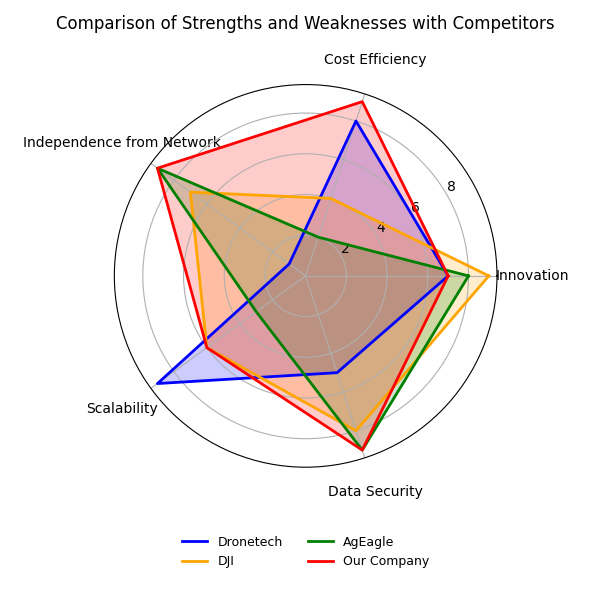
\includegraphics[width=400pt]{figures/competitors.png} 
	\caption{Comparison of Strengths and Weaknesses with Competitors}
	\source{Own illustration created with Matplotlib in Python}
	\label{fig:strengths_weaknesses} 
\end{figure}

Our ground-based \acrshort{3d} drone tracking system offers an affordable and independent solution for Austria's agricultural sector. By using calibrated ground stations with advanced image processing, we eliminate the need for expensive onboard positioning and obstacle avoidance systems. This allows to deploy simpler drones, reducing costs, maintenance complexities, and payload restrictions. As a result, small to medium enterprises can access modern drone technology, overcoming challenges like network coverage limitations and high equipment costs, making it a practical tool for improving farming operations without substantial investment.

Our approach provides several key benefits:

\begin{itemize} 
	\item \textbf{Enhanced Efficiency and Cost Savings:} Without heavy onboard sensors, drones are lighter and consume less energy, thus increasing flight times and coverage area. They can carry more payloads like seeds, fertilizers, or pesticides, enhancing operational efficiency. Reduced complexity lowers maintenance and failure risk, leading to cost savings and making precision agriculture accessible to farmers with limited budgets.
	
	\item \textbf{Secure, Independent Communication:} Our local communication system operates independently of network infrastructure, ensuring reliability in areas with connectivity issues. Unlike competitors relying on 5G, our system enhances reliability, data security, and privacy by processing tracking data locally.
	
	\item \textbf{Scalability and Flexibility:} Our ground stations can track multiple drones simultaneously without adding complexity or weight to drones. This enables scalable operations, allowing farmers to expand fleets without significant additional investment.

\end{itemize}

\section{Conclusion}

The market analysis reveals a significant opportunity for our ground-based \acrshort{3d} drone tracking system in the agricultural sector. As drone adoption in agriculture accelerates, our solution addresses key challenges like high costs, dependence on network infrastructure, and the complexity of onboard systems by eliminating the need for expensive onboard positioning, and obstacle avoidance equipment. By enabling the use of simpler, more affordable drones with increased payload capacity and simplified maintenance, we offer a unique value proposition that differentiates us from competitors relying on complex onboard technologies. Our system aligns with the needs of small to medium agricultural enterprises seeking efficient and sustainable technologies without the barriers of high initial investment and technical complexity. Further research and engagement with industry stakeholders will refine our understanding of target customers and support a successful market entry, positioning us as a competitive player in the agricultural drone market focused on accessibility and practicality.


\chapter{Solution Idea}

\section{Hardware}

\subsection{Computer}
The core idea is to perform image processing locally on each unit, thereby eliminating the need to transmit large volumes of raw image data to a central processing unit. This decentralized approach reduces the complexity of high-bandwidth data transfers and ensures that only the essential results, such as computational outputs, are transmitted. By evaluating single-board computers, the goal is to identify a cost-effective option that provides sufficient computational power for these local tasks. This approach not only streamlines data flow but also enhances scalability and independence between the stations.
% Responsible: Lukas Krahbichler

\subsection{Camera}
The selected camera must be compatible with the chosen single-board computer and provide high resolution to enable accurate tracking over greater distances. A 4K camera is proposed, as higher resolution theoretically extends the effective range of tracking. This choice balances precision and affordability, ensuring the system's effectiveness without unnecessary costs.
% Responsible: Lukas Krahbichler

\subsection{Display}
The primary station will include a display for visualizing tracked drone data. The visualization is one of the system's primary goals and will be developed as part of the programming section. The parameters for the display, such as resolution (Full HD) and size (8 to 12 inches), were secondary considerations compared to compatibility and affordability. To reduce costs, the display will only be included in the primary station, ensuring that it provides sufficient functionality for monitoring without adding unnecessary expenses.
% Responsible: Lukas Krahbichler

\subsection{Power Supply}
The proposed solution involves using an off-the-shelf power bank system to supply energy to all components, including the single-board computer, camera, display, and calibration hardware. This approach avoids the complexity of designing and building a custom battery management system, saving development time and effort. The power bank should have adequate output to power all components reliably and sufficient capacity to operate the system for a reasonable duration, although extended battery life is not a primary focus.
% Responsible: Lukas Krahbichler

\subsection{Data Transfer}
The idea is to implement local radio communication as the primary data transfer medium between the stations. This ensures independence from external networks, such as cellular systems, enhancing both security and operational reliability.
% Responsible: Lukas Krahbichler

\subsection{Calibration}
Calibration determines the relative positions and orientations of the ground stations, essential for accurate 3D drone tracking. Unlike competitors who use GNSS with RTK, this system aims to achieve similar precision through a more cost-effective and fully local approach. 

The calibration hardware, integrated onto a custom \acrfull{pcb}, could include:
\begin{itemize}
	\item Power Delivery
	\item Time-of-Flight (ToF) Laser
	\item Communication modules
	\item Stepper motors
	\item Servo motors
	\item Gyroscope/Magnetometer/Accelerometer (9DOF)
	\item End switches
	\item Microcontroller
\end{itemize}

During calibration, approximate directions could be determined using the communication system, supplemented by precise distance measurements from the ToF laser.


\section{Housing}

The initial proposition of the housing focused on following principles:
\begin{itemize}
	\item Sturdiness
	\item Size
	\item Airflow (Cooling) for the Computer
\end{itemize}

% Responsible: Prantl Niclas

\section{Programming}

\subsection{Development Environment}

A containerized Debian-based development environment is proposed to standardize dependencies and prevent system-specific issues.

\subsection{Hardware Drivers}

The software should be structured to efficiently manage hardware responsibilities.

\subsection{Calibration}
% Responsible: Lukas Krahbichler

\subsection{Camera Tracking}
Being the key element in this project, the cameras should be able to detect and track drones mid air and calculate their relative angle to the ground station. By already knowing the angle the camera is facing, this can be done by reversing the fish-eye effect of the camera and then multiplying the relative x and y position in the image by the cameras FOV.

% Responsible: Lukas Krahbichler

\subsection{Data Transfer}

% Responsible: Lukas Krahbichler

\subsection{3D Angle Calculations}
Having already calculated the relative angles for each ground station, the individual angles are being combined by using simple trigonometry. 

% Responsible: Prantl Niclas


\subsection{3D Visualization}
Operating independently from the tracking suite, the visualization system retrieves data through network sockets. It provides a comprehensive real-time display of all three ground stations and their respective cameras. When a target is detected, the system dynamically renders lines extending from each station to the target, visually representing the tracking process. Additionally, a sphere is displayed at the calculated target position, with its size indicating the accuracy of the estimation, ensuring clear situational awareness.
% Responsible: Prantl Niclas
 

\chapter{Solution}

\section{Hardware}
% Responsible: Lukas Krahbichler

\subsection{Computer}

Several single-board computers were evaluated for this project:

\begin{itemize}
	\item \textbf{NVIDIA Jetson Nano:} Offers strong \acrshort{ai} capabilities but is more expensive and exceeds project requirements \cite{nvidia_jetson_nano}.
	\item \textbf{ASUS Tinker Board S:} Affordable but lacks sufficient computational power for real-time image processing \cite{asus_tinkerboard_s}.
	\item \textbf{ArmSom Sige7 (Basic):} Balances affordability and performance, supporting necessary image processing tasks \cite{armsom_sige7}.
	\item \textbf{Raspberry Pi 4 Model B (8GB):} Well-supported but has less processing power for image processing compared to other options \cite{raspberry_pi_4b}.
\end{itemize}

The ArmSom Sige7 Basic \cite{armsom_sige7}, equipped with a Sige Active Cooling Kit \cite{armsom_sige_cooling_kit}, was chosen for its adequate performance and cost-effectiveness. However, during development, issues arose: one of the three units failed to boot, and limited documentation and support made troubleshooting difficult. In hindsight, selecting a more widely adopted platform like NVIDIA, ASUS, or Raspberry Pi would have offered greater reliability and community support.

In the end, this hardware failure was one of the main reasons the project was not fully completed, along with time constraints that prevented further troubleshooting or contacting the manufacturer, and the high costs associated with hardware replacement.

\subsection{Camera}

The camera module chosen was the 4K model from ArmSom \cite{armsom_camera_module}, specifically designed for seamless integration with the ArmSom Sige7 \cite{armsom_sige7}. This ensured full hardware compatibility and eliminated potential issues with third-party components. The module was selected for its high resolution, which allows for better tracking accuracy at greater distances. However, during testing, the camera initially produced very dark images. This was traced back to a driver issue, which was quickly resolved with support from the manufacturer.

\subsection{Display}

Initially, a 10.1-inch Full HD display from ArmSom \cite{armsom_display} was integrated into the primary station. The display was chosen for its compatibility with the ArmSom Sige7 \cite{armsom_sige7} and its reasonable price. However, as the project progressed, a redesign of the housing necessitated its removal. Redirecting the visualization to a laptop allowed for a more compact and efficient housing design.

\subsection{Power Supply}

The chosen power supply was a PD 100 W, 20,000mAh power bank from POWERADD PRO \cite{poweradd_pro_powerbank}. This model met the project's technical requirements as follows:
\begin{itemize}
	\item It supports Universal Serial Bus Power Delivery (USB-PD), essential for powering the ArmSom Sige7 \cite{armsom_sige7}.
	\item Its 100W output ensures compatibility with all connected components, including the \acrshort{pcb}.
	\item It has three ports, enabling simultaneous connections for the ArmSom board, the \acrshort{pcb}, and charging functionality.
\end{itemize}

Despite meeting these specifications, several issues arose during use. The power bank exhibited unpredictable behavior, intermittently cycling on and off. While this occurred less frequently when the power bank was fully or nearly fully charged, the problem was never completely resolved. Additionally, unexpected voltage drops were observed on the \acrshort{pcb}, with measurements showing 3.6V instead of the expected 5V from the \acrfull{usb} output. This raised concerns about power stability and its impact on system reliability. Furthermore, it is highly likely that our ArmSom computer failed due to unstable voltage levels or power spikes originating from the power bank, though this could not be definitively confirmed.

Additionally, with this setup, the station has two start buttons - one for the power bank and one for the ArmSom - which is not particularly user-friendly.

\subsection{Data Transfer}

Initially, the NRF24L01 \cite{nRF24L01} modules with \acrshort{pcb} antennas were integrated directly onto the \acrshort{pcb} to enable local radio communication between stations. However, these modules proved unreliable in the required 3-node mesh system, frequently failing to maintain stable communication.

To resolve this, the system was upgraded to NRF24L01+ PA + LNA \cite{nRF24L01_plus} modules with external antennas. This change improved signal strength but required modifications to the housing design to accommodate the larger modules. The \acrshort{pcb} remained unchanged due to the identical pinout, but the new modules were too large to be mounted directly. Instead, they had to be repositioned and connected via jumper cables.

During testing, the mesh network continued to exhibit failures or functioned only when antennas were placed in specific orientations. Further research indicated that the high transmission power of the new modules caused interference in close-range operation. Reducing the transmission power resolved these stability issues, allowing the modules to function reliably within the system.

\subsection{Calibration}

The calibration hardware ensures precise alignment and positioning of the primary and secondary stations for \acrshort{3d} tracking. Each station features a rotatable head for pitch and yaw adjustments, while roll is compensated via gyroscope measurements. Secondary stations share the same design for simplicity, but only the primary station includes a \acrshort{tof} laser for precise distance measurement. Secondary stations rely on camera-based alignment.

\subsubsection*{Components and Functionality}

\paragraph{Rotatable Head (Pitch and Yaw Axes):}
The system uses compact 28BYJ-48 stepper motors controlled via ULN2003 driver boards \cite{angeek_28byj_48}. The used end-switches from InduSKY \cite{indusky_microswitch} are configured in normally closed mode to detect faults like loose connections. Servos \cite{miuzei_servos} were initially considered but dismissed due to cost, size, and complexity.

\paragraph{Gyroscope and Compass:}

Initially, we attempted to use a \textbf{9DoF sensor module} \citep{jwbl_dof_sensor} that integrated a 3-axis 12-bit accelerometer, a 3-axis earth magnet sensor, and a 3-axis 16-bit gyroscope. However, the gyroscope did not function at all, while the accelerometer and magnetometer failed to provide correct data. The earth magnet sensor, in particular, delivered inconsistent readings, fluctuating significantly between measurements and rendering it unreliable for absolute orientation.

As a result, we switched to a \textbf{GY-521 gyroscope} \cite{azdelivery_gy_521}, which provides 6-axis data for tilt measurement and alignment correction. Additionally, a \textbf{GY-271 compass} \cite{azdelivery_gy_271} was initially included for absolute orientation but was later abandoned due to unreliable calibration and inconsistent results. The compass remains on the \acrshort{pcb} but is not actively used in the system.

\paragraph{ToF Laser Module:}
The primary station features a DFRobot Infrared Laser Distance Sensor \cite{dfrobot_ir_sensor} with a 5 centimeters to 80 meters range and millimeter-level accuracy. It is used for precise distance measurements and requires an unobstructed line of sight between the stations.

\paragraph{Camera for Visual Alignment:}
Each station’s 4K camera \cite{armsom_camera_module} identifies and aligns with other stations during calibration. The cameras should track the bright orange secondary stations for positioning, replacing the originally planned but unreliable radio-based direction-finding approach with Long Range (LoRa) modules \cite{tecnoio_lora_modules}.

\paragraph{\acrshort{pcb}:}
The calibration system relies on a custom-designed \acrshort{pcb} to integrate various components necessary for precise positioning and alignment. The \acrshort{pcb} was designed using \textbf{Altium Designer 22.11.1} \cite{altium_designer_22}, with components sourced from \textbf{DigiKey} \cite{digikey} and the board itself manufactured by \textbf{JLCPCB} \cite{jlcpcb}. Assembly was completed both in the school’s workshop and at home.

The \acrshort{pcb} incorporates an \textbf{Arduino Nano} by DFRobot \cite{arduino_nano_dfrobot} as the main microcontroller. However, during development, we encountered program storage limitations, restricting the complexity of the firmware. In hindsight, selecting a microcontroller with more program storage, such as the \textbf{Arduino Uno R3} \cite{arduino_uno_dfrobot}, would have provided more flexibility and prevented these constraints.

\textbf{Key Functions of the \acrshort{pcb}:}
\begin{itemize}
	\item Provides power distribution to the calibration components.
	\item Interfaces with the stepper motor drivers for head rotation control.
	\item Integrates the gyroscope, compass, and \acrshort{tof} laser module.
	\item Facilitates Light Emitting Diode (LED) indicators for status feedback.
\end{itemize}

\textbf{Issues Encountered During Development:}
\begin{itemize}
	\item The \textbf{\acrshort{usb} input connector} was never soldered because the cable would not fit inside the housing. Instead, wires were directly soldered to the board.
	\item The \textbf{Arduino orientation} was incorrect in Altium, resulting in the microcontroller being mounted in the opposite direction than originally planned. This led to changes in cable management in the housing design.
	\item The \textbf{LED on/off switching functionality} did not work as intended, requiring two additional manual connections to be made on each \acrshort{pcb}.
	\item The \textbf{Communication between the Arduino Nano \cite{arduino_nano_dfrobot} and the ArmSom Sige7 \cite{armsom_sige7}} was initially planned via Inter-Integrated Circuit (I2C). However, this did not work as expected. After unsuccessful troubleshooting attempts, we switched to Universal Asynchronous Receiver Transmitter (UART) communication. This change caused issues with the camera, as both systems could not run simultaneously. Ultimately, we resolved this by using a direct \acrshort{usb} connection, running a cable from a \acrshort{usb}-A port on the ArmSom board to the Micro-\acrshort{usb} port on the Arduino Nano.
\end{itemize}

Despite these issues, the \acrshort{pcb} successfully serves as the central interface for calibration hardware, integrating all necessary sensors and controllers to facilitate the calibration process.

\subsubsection*{Calibration Hardware Conclusion}
While the calibration system was designed to reduce costs compared to \acrshort{gnss} with \acrshort{rtk}, the final implementation became expensive. In hindsight, the cost was close to that of \acrshort{rtk}-based alternatives used by competitors.

\section{Housing}
\subsection{First Version}  

The initial housing design was developed before all hardware components were physically available, relying exclusively on online specifications and manufacturer-provided measurements. While this approach enabled early prototyping, it also introduced dimensional inaccuracies. One of the most notable issues was an incorrectly sized display cutout, which required significant adjustments and a complete reprint of the housing.  

As the project progressed, multiple redesigns became necessary to refine the housing’s functionality and accommodate unforeseen challenges.

\paragraph{Adaptation to Hardware Changes}  
As final hardware selections were made, modifications were required to ensure a proper fit for all components. Throughout the development process, some components were replaced or upgraded, necessitating corresponding adjustments to the housing design. This iterative approach ensured compatibility with the latest hardware configurations while maintaining structural integrity.  

\paragraph{Improved Accessibility}  
To facilitate maintenance and future modifications, internal components needed to be more easily accessible. Several design refinements were implemented, including repositioning mounting points, enlarging access openings for connectors, and improving ventilation. These changes simplified servicing and upgrades, reducing downtime and enhancing long-term usability.  

\paragraph{Simplified Assembly and Structural Refinements}  
Initial prototypes were complex and time-consuming to assemble. To address this, the design was incrementally refined to minimize the number of assembly steps and reduce the likelihood of errors. Additionally, the housing was structured as a modular system, consisting of multiple interlocking parts. This approach optimized printability within standard \acrshort{3d} printing constraints while also enhancing maintainability, as individual sections could be replaced or upgraded without requiring a complete reprint.  

\paragraph{Key Design Challenges and Iterative Improvements}  
Throughout development, several specific design challenges emerged, necessitating further refinements:  
\begin{itemize}  
	\item \textbf{Countersinks:} Initially too small, requiring adjustments based on print quality to ensure proper screw seating.  
	\item \textbf{Screw Holes:} Some holes were oversized, allowing screws to spin freely instead of securing properly. This was addressed by refining tolerances for a precise fit.  
	\item \textbf{Tolerance Adjustments:} Various fitment issues arose due to minor dimensional inaccuracies, requiring iterative refinements to achieve optimal compatibility between components.  
	\item \textbf{Ventilation:} Early prototypes lacked sufficient airflow, increasing the risk of overheating. Ventilation openings were expanded and repositioned to enhance cooling efficiency.  
	\item \textbf{Structural Stability:} Additional reinforcements were implemented to ensure that the housing could withstand vibrations and external forces during operation.  
	\item \textbf{Hardware Integration:} Mounting positions were refined to simplify the integration of components, improving ease of assembly and overall usability.  
	\item \textbf{Port Accessibility:} The layout was adjusted to provide better access to the computer’s ports, simplifying connectivity.  
\end{itemize}  

These continuous iterations and refinements allowed the first version of the housing to evolve into a more practical and functional design. The lessons learned from this phase directly influenced subsequent iterations, leading to an optimized final version.  
  
  
\subsection{Second (Final) Version}
Building upon the insights gained from the first housing iteration, the second version introduced several key improvements to enhance functionality, maintainability, and overall design efficiency.  

\paragraph{Enhanced Modularity and Accessibility}  
A major focus of the redesign was to improve modularity, simplifying both assembly and maintenance. The revised structure allows for more efficient disassembly, significantly reducing the time required for maintenance and hardware adjustments. Additionally, hardware accessibility was prioritized, ensuring that critical components could be reached without excessive disassembly.  

\paragraph{Compact and Optimized Design}  
One of the most impactful changes was the removal of the display, which had previously dictated the dimensions of the housing. This adjustment enabled a more compact and streamlined design, optimizing space utilization while maintaining full functionality. Despite these structural changes, the motor mechanism from the first version was retained, reducing development time and ensuring continuity in core functionalities.  

\paragraph{Redesigned Bottom Section}  
The bottom section of the housing, which accommodates essential components such as the \acrshort{pcb}, computer, power bank, and cooling system, underwent a complete redesign. This revision focused on improving organization, airflow, and ease of access to internal hardware, ensuring more efficient operation and maintenance.  

\paragraph{Integration of Threaded Inserts}  
To enhance durability and improve the reliability of screw connections, threaded inserts were introduced. These additions provide several benefits:  
\begin{itemize}  
	\item Increased longevity of screw mounts, preventing wear and deformation over multiple assembly cycles.  
	\item Simplified disassembly and reassembly, facilitating faster maintenance and upgrades.  
	\item Enhanced structural integrity, ensuring that fastening points remain secure over time.  
\end{itemize}  

\paragraph{Yaw Motor Issue \& Gear System Upgrade}  
During testing, the initial yaw motor was found to be underpowered, resulting in performance limitations. To address this issue, a gear system was implemented to increase torque, enabling smoother and more reliable movement. This upgrade ensured that the system could operate effectively under varying conditions without compromising precision or stability.  

\paragraph{Refinements to the Bottom Section}  
Even after the major redesign, additional modifications were necessary to further optimize the housing’s performance and durability:  
\begin{itemize}  
	\item Improved interconnections between housing parts, enhancing structural integrity.  
	\item Optimized airflow channels to improve cooling efficiency and prevent overheating.  
	\item Increased overall stability to withstand vibrations and external forces.  
	\item Adjusted hardware mounting positions for seamless integration and accessibility.  
	\item Enhanced access to the computer’s ports, ensuring convenient connectivity.  
	\item Redesigned power button mechanism for a more intuitive and reliable user interface.  
\end{itemize}  

By incorporating these refinements, the second housing version achieved a significant leap in reliability, ease of use, and long-term maintainability, making it better suited for real-world deployment.  

\subsection{3D Printing Process}  

The housing components were fabricated using a \textbf{Bambu Lab P1S} \acrshort{3d} printer, chosen for its high-speed printing capabilities and reliable output quality. The material selection varied throughout the development phase to balance rapid prototyping needs with long-term durability requirements.  

\paragraph{Prototyping with PLA}  
During the initial prototyping stage, \textbf{\acrfull{pla}} was used due to its ease of printing and fast turnaround time. This enabled rapid iteration and testing of design modifications without significant material costs. However, \acrshort{pla}'s mechanical properties and limited environmental resistance made it unsuitable for the final application.  

\paragraph{Final Production with PETG}  
For the final version, \textbf{\acrfull{petg}} was selected due to its superior durability, higher temperature resistance, and suitability for outdoor conditions. Unlike \acrshort{pla}, \acrshort{petg} offers improved impact resistance and reduced brittleness, ensuring a more robust enclosure for long-term use.  

\paragraph{Considerations for Printing with PETG}  
Although \acrshort{petg} generally requires longer print times and careful tuning compared to \acrshort{pla}, the use of \textbf{High-Flow (HF)} filament allowed for efficient production without a significant increase in cost or time. To ensure optimal print quality, \acrshort{petg} filament was dried for \textbf{eight hours} in a filament dryer before printing. This step was necessary to prevent moisture absorption, which can negatively impact layer adhesion and overall print strength.  

By leveraging the strengths of both materials at different development stages, the housing design was iteratively refined while maintaining efficiency in the fabrication process.

% Responsible: Prantl Niclas

\section{Programming}
\subsection{Development Environment}  

To facilitate efficient and consistent development of the Armsom codebase, a \textbf{custom development environment} was created. This environment builds upon and extends the previously developed system by French Bakery \cite{fb_dev_environment}, incorporating various improvements to enhance usability, maintainability, and cross-platform compatibility.  

\paragraph{Containerized Development Approach}  
A \textbf{Debian-based development container} was employed to provide a standardized environment for \textbf{C++ development and cross-compilation}. By using containerization, all necessary dependencies, libraries, and toolchains are encapsulated within a controlled environment, ensuring that every developer operates under identical conditions, regardless of the underlying host system.  

\paragraph{Cross-Platform Consistency}  
One of the primary motivations for adopting a containerized approach was the need to support development across multiple systems, each running different operating systems. Without a uniform environment, discrepancies in library versions, compiler behavior, and system dependencies could introduce inconsistencies, leading to potential compatibility issues. By utilizing a \textbf{Debian-based development container}, the project ensures:  
\begin{itemize}  
	\item \textbf{Improved Repeatability:} Code behaves identically across all development machines, eliminating system-dependent discrepancies.  
	\item \textbf{Stable and Predictable Development Workflow:} Developers can work with a predefined toolset, reducing setup time and potential conflicts.  
	\item \textbf{Seamless Cross-Compiling:} The containerized approach streamlines cross-compilation, allowing code to be developed on one system while being compiled for another target architecture.  
\end{itemize}  

By leveraging this structured development environment, the project benefits from enhanced collaboration, reduced debugging overhead, and a more streamlined deployment process. This approach not only improves efficiency but also ensures long-term maintainability and scalability of the development workflow.  

\subsection{Hardware Drivers}
A significant portion of the software development effort was dedicated to implementing robust and efficient hardware drivers. These drivers facilitate seamless communication between various hardware components and ensure reliable operation of the system. The hardware control is primarily divided between two processing units: the \textbf{Armsom} (main computer) and the \textbf{Arduino Nano}, each responsible for different aspects of device management.

\begin{itemize}
	\item \textbf{Armsom (Main Computer)}
	\begin{itemize}
		\item Stepper motor drivers
		\item Serial communication with Arduino Nano
	\end{itemize}
	\item \textbf{Arduino Nano}
	\begin{itemize}
		\item RF24 Mesh networking
		\item \acrfull{pwm}-based fan control
		\item \acrshort{tof} laser module
		\item Compass and gyroscope integration
		\item Communication with the Armsom
	\end{itemize}
\end{itemize}

\paragraph{Armsom}
The Armsom is responsible for controlling the stepper motors, ensuring precise movement across both horizontal and vertical axes. A dedicated stepper driver interface provides comprehensive support for various motion parameters, including:
\begin{itemize}
	\item Half-stepping and gear ratio compensation for smooth motion.
	\item Absolute and relative positioning in both steps and angular degrees.
	\item Speed control with acceleration management.
	\item Continuous positional awareness to maintain accurate alignment.
\end{itemize}

To establish a robust communication link with the Arduino Nano, a serial interface was developed, incorporating acknowledgment mechanisms to ensure reliable data transmission. This approach verifies the successful execution of commands and prevents the loss of critical control signals. While the Armsom serves as the central processing unit, it interacts with key hardware components—such as the cooling fan, sensors, and RF24-based networking modules—indirectly through the Arduino Nano, which acts as an intermediary for hardware control and data acquisition.

\paragraph{Arduino Nano}
The Arduino Nano is responsible for handling auxiliary hardware tasks and serves as a bridge between the Armsom and various peripheral components.

\subparagraph{RF24 Mesh Networking}
The RF24 Mesh protocol provides reliable wireless communication between ground stations. The implementation ensures efficient data transfer and message routing across the mesh network. For further details, refer to Section~\ref{subsec:DataTransfer}.

\subparagraph{PWM Fan Control}
A simple \acrshort{pwm} control system is used to regulate the cooling fan speed. The fan is controlled via a single PWM pin, enabling dynamic adjustments based on temperature or other system conditions.

\subparagraph{ToF Laser}
The \acrshort{tof} laser module is responsible for distance measurements station alignment. A custom serial-based communication interface was developed due to limitations in existing libraries, providing additional functionalities such as:
\begin{itemize}
	\item Checksum validation for data integrity.
	\item Adjustable range and resolution settings.
	\item Laser diode power control (on/off).
	\item Automatic re-request mechanism in case of transmission errors.
\end{itemize}

\subparagraph{Serial Communication with Armsom}
A dedicated serial communication link between the Arduino Nano and the Armsom allows efficient data exchange. Key features of this communication system include:
\begin{itemize}
	\item Buffered message storage for incoming network data until requested by the Armsom.
	\item Memory-efficient design to account for the Nano’s limited random access memory (RAM) capacity.
	\item Integrated debugging capabilities, enabling the Nano to send diagnostic data to the Armsom’s command-line interface (CLI).
\end{itemize}

This modular hardware driver implementation ensures stable, reliable, and maintainable operation across all system components.

%Responsible: Niclas Prantl

\subsection{Calibration}
% Responsible: Lukas Krahbichler

The calibration process was only implemented in a basic form. Only tests were made, where the relative positions of the stations had to be manually input by the user, after which the laser was used to measure distances. Due to our critical hardware failures, further development towards automation was not possible. While the conceptual framework was outlined, practical validation and refinement beyond manual calibration could not be completed.

\subsection{Camera Tracking}
% Responsible: Lukas Krahbichler

The implementation of the camera tracking system progressed to the conceptual and initial development stages. The approach described in the solution idea was outlined, and preliminary considerations were made regarding tracking accuracy and computational feasibility. However, due to hardware constraints, further refinement and real-world validation could not be completed within the project's timeframe.

\newpage
\begin{figure}[H]
	\subsection{Data Transfer} \label{subsec:DataTransfer}
	\centering
	\begin{minipage}{0.5\textwidth} % Text on the left
		\raggedright % Aligns text to the left
		\paragraph{Protocol Overview:}
		
		To ensure reliable and efficient data transmission, a structured JSON-based communication protocol was developed. Each message is encapsulated in a \textbf{parent message}, containing a type, unique \acrfull{id}, and timestamp. The message type can be one of the following:
		
		\begin{itemize}
			\item \textbf{req} – Requests information or an action.
			\item \textbf{ack} – Confirms successful execution of an action.
			\item \textbf{repl} – Provides responses to requests.
			\item \textbf{data} – Transmits tracking or station-related information.
		\end{itemize}
		
		with each message type having a specified schema. In case the message type is \textbf{data}, it can be further separated in:
		
		\begin{itemize}
			\item \textbf{Target Result (tres)}: Contains object tracking data, including camera angles and object \acrshort{id}s.
			\item \textbf{\acrshort{3d} Target Result (tres3)}: Extends \textbf{tres} with precise \acrshort{3d} position.
			\item \textbf{Station Information (sinf)}: Provides metadata on ground stations, including position, direction, and camera specifications.
		\end{itemize}
		
		\paragraph{Protocol Advantages:} \
	
		The protocol ensures:
		\begin{itemize}
			\item \textbf{Efficiency}: Predefined schemas enable fast parsing and low-latency communication.
			\item \textbf{Scalability}: The modular design allows for future extensions.
			\item \textbf{Reliability}: The acknowledgment system provides valuable feedback for error handling.
		\end{itemize}
		
		This structured approach enables seamless coordination between ground stations, visualization tools, and tracking algorithms.
		
	\end{minipage}%
	\hfill
	\begin{minipage}{0.38\textwidth} % Image on the right
		\centering
		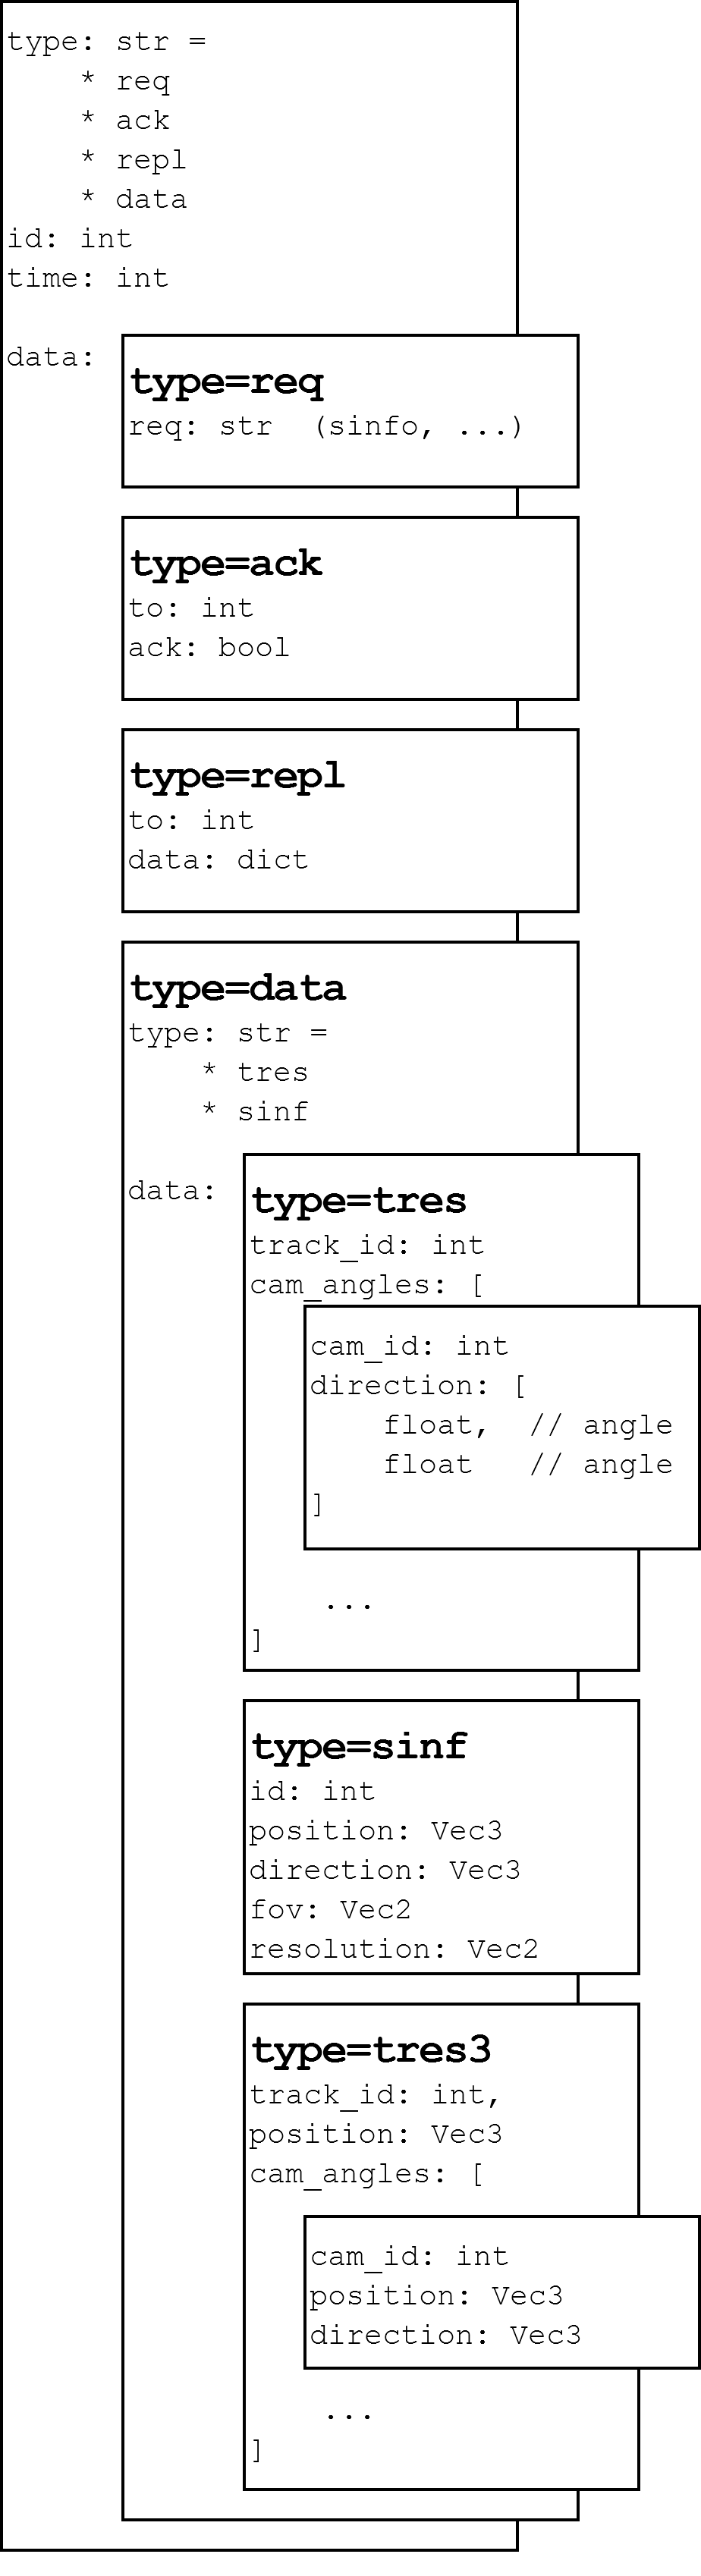
\includegraphics[width=\textwidth]{figures/SS_Protocol_Message}
		\caption{Message Structure}
		\source{Own illustration created with Draw.io}
		\label{fig:ssprotocolmessage}
	\end{minipage}
\end{figure}

\paragraph{Theoretical Solution:}  
To establish a robust and efficient communication framework, all three ground stations are integrated into a \textbf{Mesh network}, where the \textbf{primary station} assumes the role of the central server, while the \textbf{secondary stations} operate as clients.

During system initialization, the primary station enters a \textbf{standby state}, waiting for all secondary stations to establish a connection. Once all connections are confirmed, the system initiates a calibration procedure, synchronizing positional data and aligning reference frames to ensure precise tracking and analysis.  

For standard operation, the primary station transitions into a \textbf{listen-only mode}, except for sending essential acknowledgments. This strategic design significantly reduces computational overhead and minimizes RAM usage, allowing the system to maintain high efficiency even under demanding conditions. By limiting active processing on the primary station, the architecture optimizes real-time data handling while ensuring rapid and reliable communication between all networked components.  

This approach not only enhances the system's scalability but also improves fault tolerance by enabling seamless reconnections in case of temporary communication disruptions.  

\paragraph{Code Implementation:}  
The implementation of the communication framework was significantly streamlined by leveraging the \texttt{RF24Network} and \texttt{RF24Mesh} libraries, which provide a robust abstraction layer for interfacing with the \texttt{NRF24L01+ PA + LNA} modules. These libraries handle much of the low-level networking functionality, including packet routing, automatic retransmissions, and dynamic addressing, thereby reducing development complexity and allowing for a more structured and maintainable architecture.  

However, to fully integrate the system’s requirements, a modular software interface needed to be developed, capable of supporting both \textbf{server} (primary station) and \textbf{client} (secondary station) nodes. This involved designing a flexible communication framework that could dynamically handle various message types, manage connections efficiently, and ensure reliable data transfer.  

A key aspect of the implementation was integrating the previously defined \textbf{custom network protocol}, which structures and organizes all transmitted data. The protocol was designed to handle distinct message types, including requests, replies, acknowledgments, and data transmissions. Within data messages, further categorization enables the transmission of tracking results and station-specific information.  

By adopting this structured approach, the system benefits from improved scalability, reduced processing overhead, and enhanced reliability, making it well-suited for real-time applications with stringent performance requirements.  

% Responsible: Lukas Krahbichler

\subsection{3D Angle Calculations}
\paragraph{Approach:}
In contrary to the initially proposed "simple trigonometry", the calculations are being done using an approximation algorithm. This approach was chosen, because the vectors from each station to the target will never be fully accurate, so in the real world the three Vectors would never meet, which makes solving it using trigonometry impossible. Approximation works, by specifying a "rule set" (a function returning an integer) and trying to achieve the lowest possible output value, using a three dimensional position as input parameter. 

\paragraph{Code Solution:}
In Python, this approximation is performed using \\ \texttt{scipy.optimize.minimize}. The objective function calculates the sum of distances to each line, with lower values indicating points closer to the center of the vector system. The second parameter, \texttt{x0}, defines the starting point for the approximation algorithm, set as the center of our coordinate system, which coincides with the center of our ground station array. Since this function also depends on \texttt{lines}, it must be provided as an argument in \texttt{minimize}. Additionally, the fourth parameter, \texttt{method}, is specified as \texttt{"BFGS"}.

\textbf{Broyden–Fletcher–Goldfarb–Shanno algorithm:} \\
The Broyden–Fletcher–Goldfarb–Shanno (BFGS) algorithm is an iterative method for solving unconstrained nonlinear optimization problems. It preconditions the gradient with curvature information, gradually approximating the Hessian matrix using a generalized secant method. Unlike Newton’s method, BFGS avoids matrix inversion, reducing computational complexity to O(n2)O(n2) instead of O(n3)O(n3). The L-BFGS variant is efficient for large-scale problems, while BFGS-B handles box constraints. Named after Broyden, Fletcher, Goldfarb, and Shanno, it remains widely used in numerical optimization.\citep{BFGS_wiki}

\hspace*{-1.2cm}

\begin{lstlisting}[caption={Example of 3D Angle Calculation}, label={lst:exampleCalculation}, style=PythonStyle]
lines: list[tuple[np.array, np.array]] = ...


def objective(
	point: np.array,
	lines: list[tuple[np.array, np.array]]
) -> float:
	"""
	calculate the sum of the distances to each line
	"""
	return sum(distance_to_line(
		point, line[0], line[1]
	) for line in lines)


result = minimize(
	objective,
	x0=np.array([0.0, 0.0, 0.0]),
	args=(lines,),
	method='BFGS'
)
\end{lstlisting}

\begin{figure}[H]
	\centering
	\hspace*{-1.5cm} 
	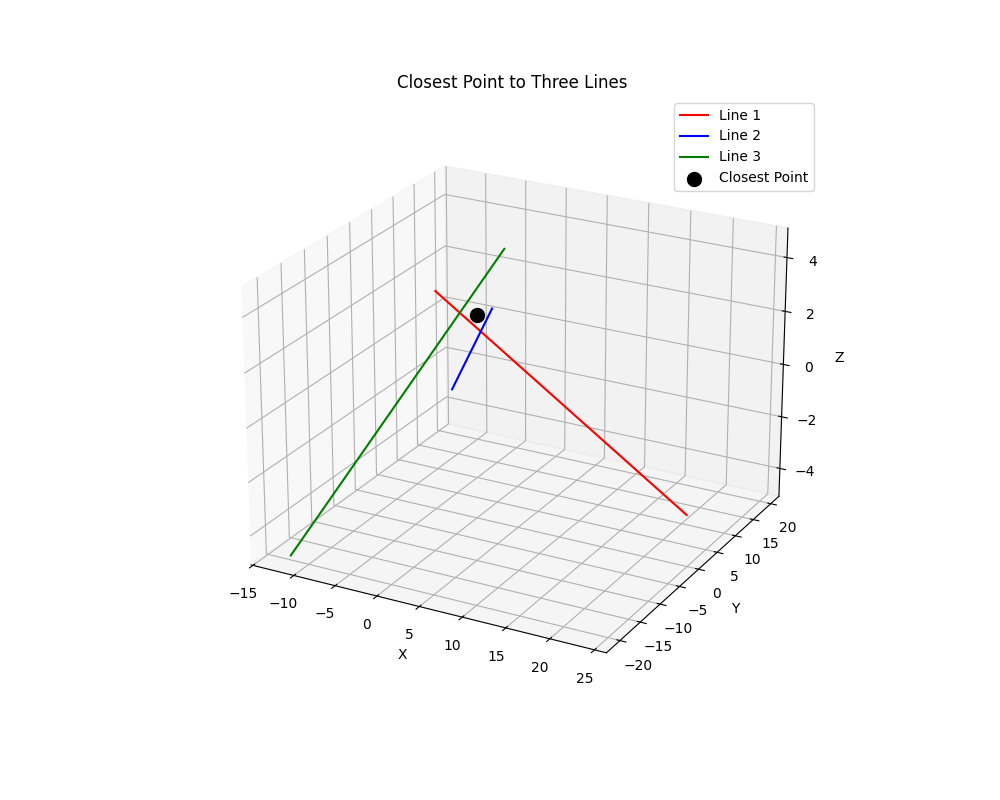
\includegraphics[width=400pt]{figures/approximation_algorithm}
	\caption{Example Visualization of the algorithm}
	\source{Own illustration created with Matplotlib in Python}
	\label{fig:approximationalgorithm}
\end{figure}

As shown in the illustration above, when given three lines in random orientations, the algorithm successfully identifies their center. Testing revealed that the code executes in approximately 400 to 600 µs, which is more than fast enough for our use case.

\paragraph{Tracking}
To enhance target tracking, each identified object is assigned a unique 'track \acrshort{id},' which allows it to be consistently identified at any given time. Additionally, every calculated position of the object is recorded throughout its movement. This comprehensive data logging makes it possible to fully reconstruct the object's flight path, providing a detailed history of its trajectory and enabling further analysis if needed.

% Responsible: Prantl Niclas

\subsection{3D Visualization}
\paragraph{Network Protocol}  
To ensure broad compatibility and accessibility, the visualization application was designed to run on a wide range of devices, including user-provided hardware. As a result, a dedicated network communication protocol was required to facilitate seamless data exchange between the tracking system and the visualization client.  

To achieve this, the previously defined network protocol was not only reused but also further refined and optimized for this specific application. Unlike a purely request-based system, the server is also capable of broadcasting updates autonomously, ensuring that clients receive critical tracking information in real time. This hybrid approach balances efficiency and responsiveness, allowing visualization clients to both request specific data when needed and passively receive updates without constant polling.  

The refined protocol structure enables the efficient transmission of tracking and calibration data while minimizing network overhead. The updated communication procedure is outlined below:  

\begin{figure}[H]
	\centering
	\hspace*{-1.5cm}
	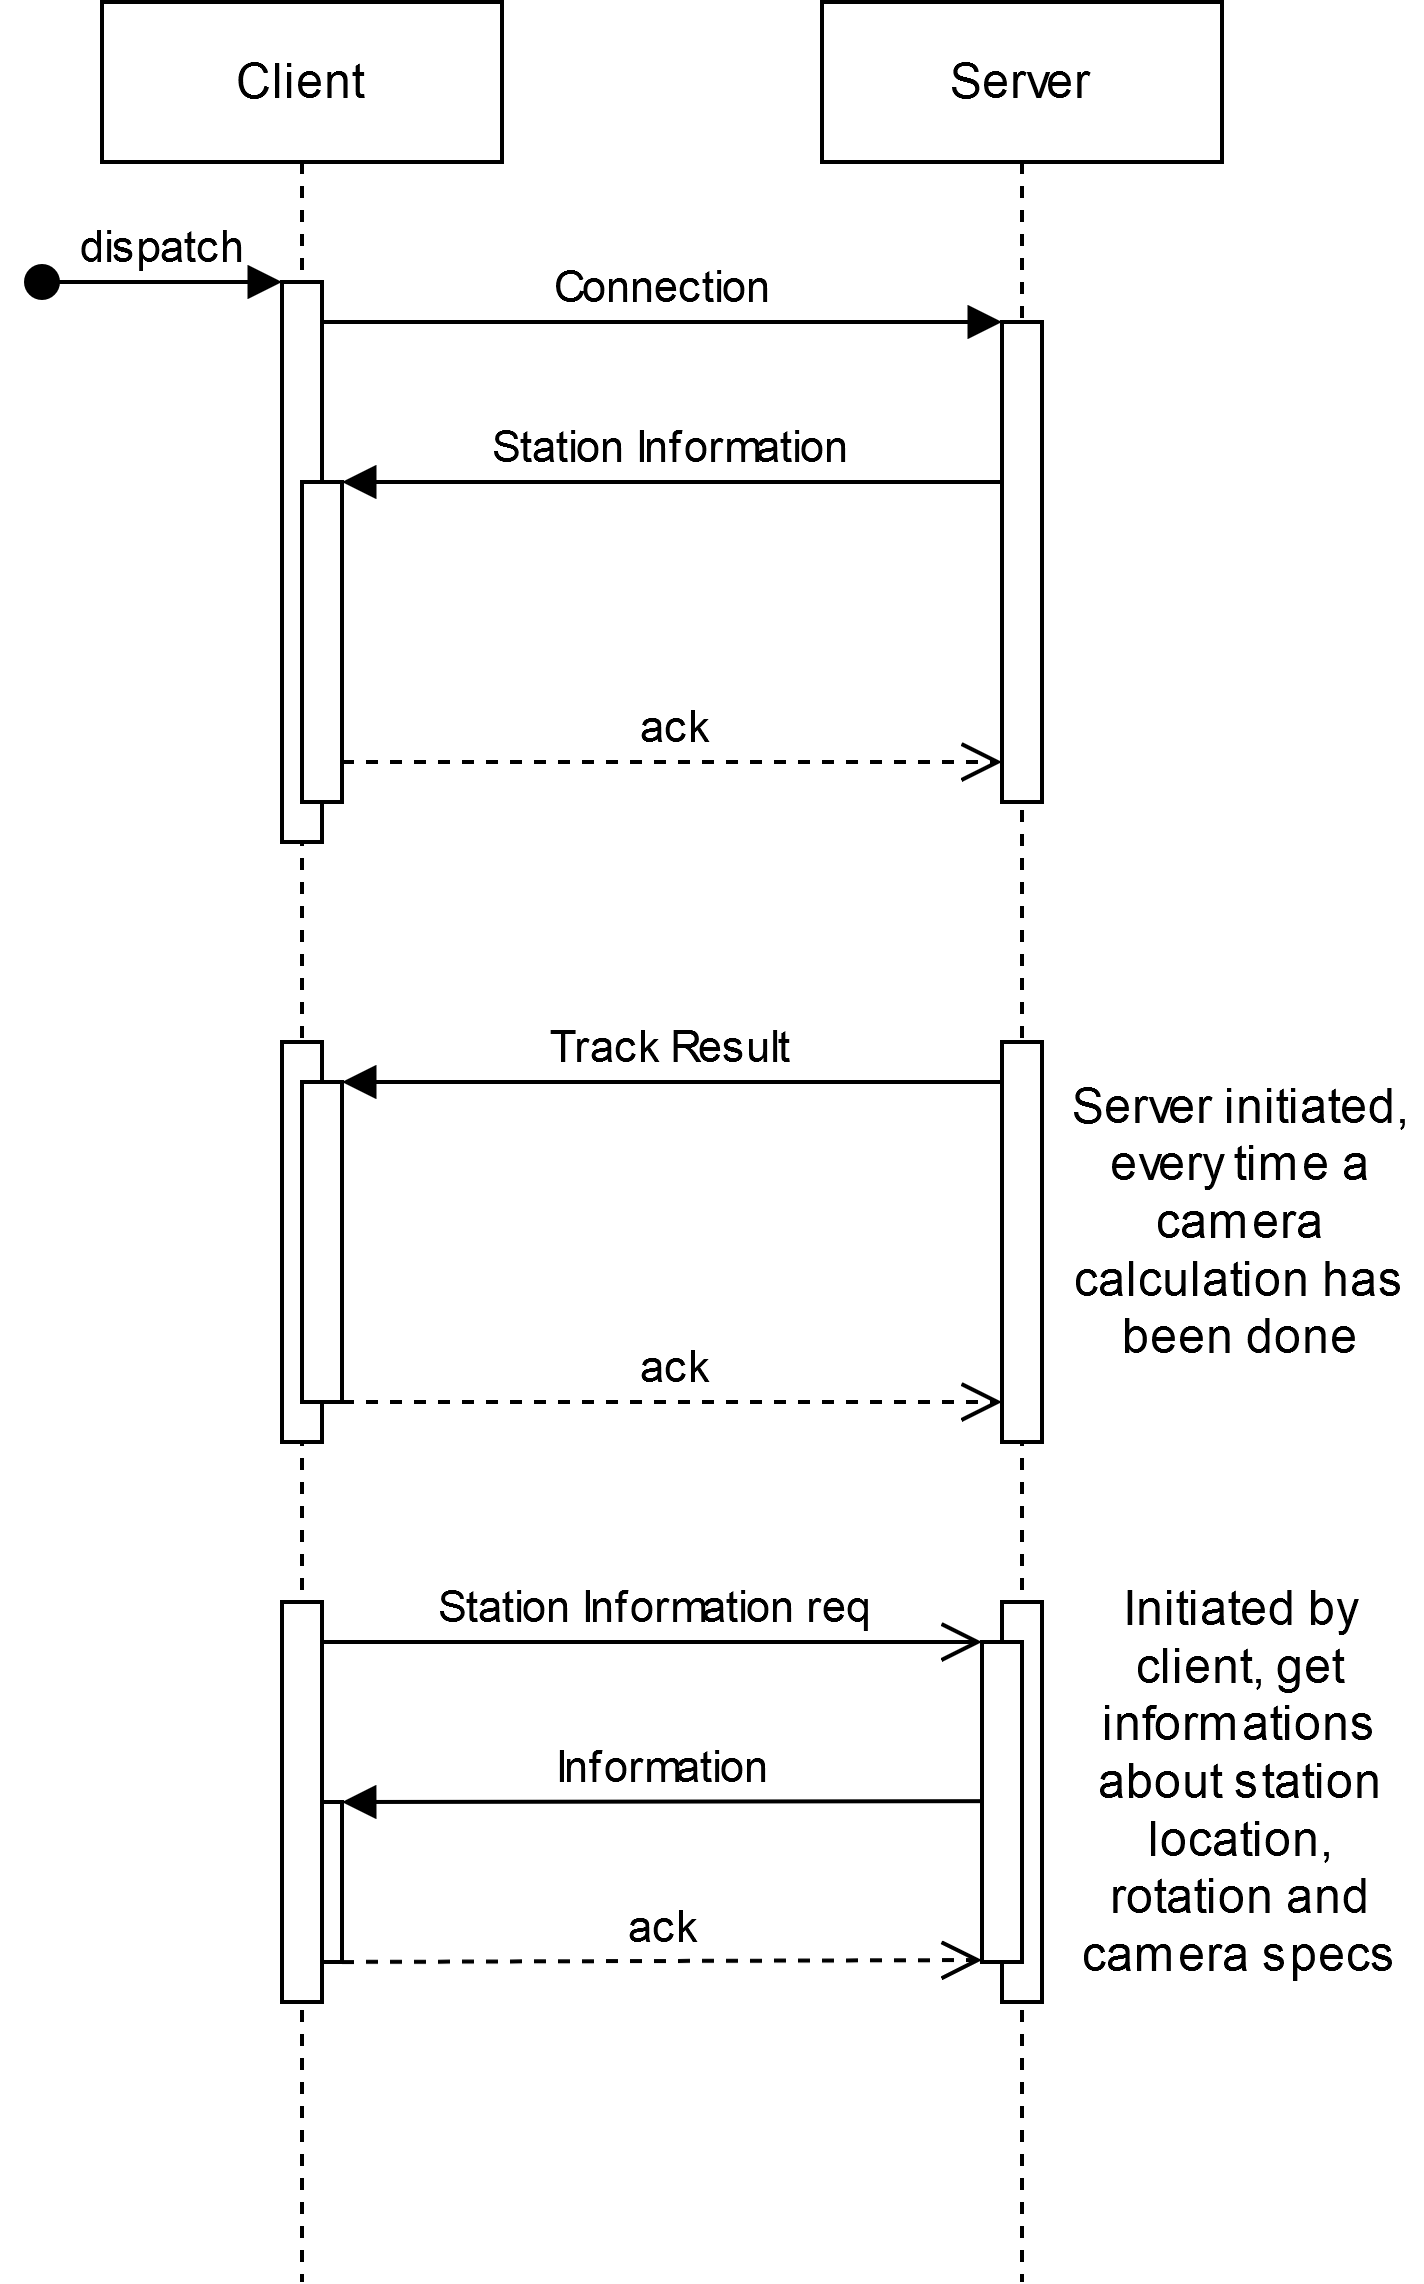
\includegraphics[width=220pt]{figures/SS_Protocol}
	\caption{Simplified Network Protocol}
	\source{Own illustration created with Draw.io}
	\label{fig:ssprotocol}
\end{figure}

\paragraph{Rendering Engine}
Given that the \acrshort{3d} tracking component was already developed in Python, it was a logical decision to implement the visualization system in Python as well to maintain consistency and streamline integration. For this purpose, I selected \textbf{Ursina}, a lightweight yet powerful \acrfull{3d} rendering engine designed for Python. My prior experience with \textbf{Ursina} further reinforced this choice, as it enables the efficient rendering of simple \acrshort{3d} models with minimal development overhead. Its intuitive API and ease of use makes it well-suited for rapidly prototyping and displaying real-time visualizations while ensuring smooth performance.

% Responsible: Prantl Niclas

 
\chapter{Conclusion}

\chapter*{Acknowledgments}

We would like to express our deepest gratitude to our supervising teachers, Professor Götsch, Professor Egger, and Professor Jank, for their invaluable guidance, insightful feedback, and unwavering support throughout the development of this thesis.

We are also profoundly thankful to our families for their continuous support, both emotionally and financially, which has made it possible for us to pursue our education at this institution. Living away from home during the week in a *Schülerheim*, due to the significant distance from our school, has presented its own set of challenges.

Lastly, we extend our appreciation to our classmates and friends who have been a source of inspiration and assistance throughout this project.



% 
\chapter{Latex-Beispiele}
\label{chap:bsp}

\section{Aulistungen}

\begin{itemize}
	\item \textit{Kursiv} Text 1
	\item \textbf{Fett}  
	\item \texttt{TT} 
	\end{itemize}
	
	Dasselbe durchnumeriert:
	
	\begin{enumerate}
		\item \textit{Kursiv} Text 1
		\item \textbf{Fett}  
		\item \texttt{TT} 
	\end{enumerate}


\section{Tabellen}

Eine Tabelle mit Testdaten:


\begin{table}[H]
	\begin{center}
		\begin{tabular}{lrrrrr}\hline\hline
			\multicolumn{1}{l}{\textbf{position}}&
			\multicolumn{1}{c}{\textbf{mean}}&
			\multicolumn{1}{c}{\textbf{median}}&
			\multicolumn{1}{c}{\textbf{sd}}&
			\multicolumn{1}{c}{\textbf{min}}&
			\multicolumn{1}{c}{\textbf{max}}
			\\ \hline
			\textbf{6}&$6.89$&$5.61$&$ 7.29$&$0.31$&$160.12$\\
			\textbf{9}&$5.35$&$4.39$&$ 4.94$&$0.18$&$ 76.40$\\
			\textbf{12}&$8.70$&$6.96$&$10.72$&$0.15$&$239.88$\\
			\textbf{13}&$9.01$&$7.54$&$ 7.60$&$0.15$&$138.86$\\
			\textbf{15}&$8.18$&$6.99$&$ 6.86$&$0.16$&$117.26$\\
			\textbf{16}&$5.26$&$4.42$&$ 4.99$&$0.08$&$110.21$\\
			\textbf{17}&$5.87$&$4.79$&$ 6.13$&$0.15$&$ 98.88$\\
			\textbf{36}&$8.21$&$6.72$&$ 7.58$&$1.36$&$122.35$\\
			\textbf{42}&$6.77$&$5.93$&$ 6.98$&$1.72$&$123.72$\\
			\textbf{43}&$6.27$&$5.53$&$ 3.21$&$0.57$&$ 35.69$\\
			\hline
		\end{tabular}
	\end{center}
	\caption{Eine Tabelle mit Testdaten} 
	\label{tabelle:test}
\end{table}

Sprachen wie z.B. \textbf{R} können Latex-Tabellen exportieren, sie müssen also nicht immer so aufwändig formatiert werden.			


\section{Abbildungen}

 \begin{figure}[H]
 	%\centering
 	\hspace*{-1.5cm}
 	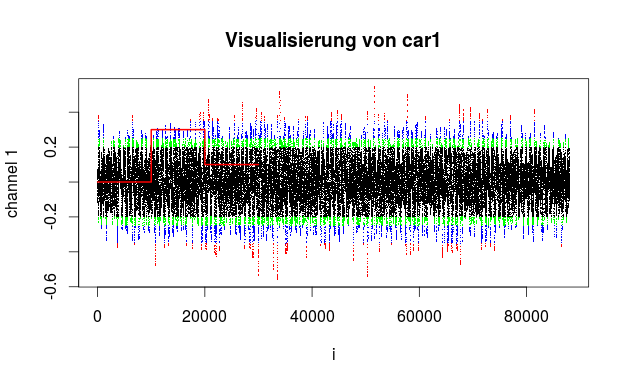
\includegraphics[width=512pt,height=280pt]{figures/bsp.png}
 	\caption{Ein Beispiel für ein Bild}
 	\label{bild:beispiel}
 \end{figure}
 
 
\section{Quellcode}

Quellcode wird automatisch (mit der Möglichkeit die Sprache anzugeben) formatiert und in das Listings-Verzeichnis gegeben:

\subsection{Java-Code}

\begin{lstlisting}[style=Java, caption={Java-Beispiel}, captionpos=b]
int i = 1;
float f = 2;
System.out.printf("Int-Z %d Float-Z: 52f",i ,f );
\end{lstlisting} 


\subsection{Python-Code}
 
\begin{lstlisting}[style=Python, caption={Python-Beispiel}, captionpos=b]
#Hier ein kleines Beispiel in Python
lower = 0
upper = 10
for i in range(lower,upper):
print(i)
\end{lstlisting} 


\subsection{Lesen von Dateien}
 
Es kann auch direkt von Dateien gelesen werden:

\lstinputlisting[style=Java, label={java_bsp}, caption={Java-Beispiel von Datei}, captionpos=b]{sourcecode/First.java}
 
\section{Referenzen}
			
Beispiele für die Verwendung von Referenzen: 

\begin{itemize}
	\item Wie in Tabelle ~\ref{tabelle:test} ersichtlich... 
	\item Wir sind im Kapitel ~\ref{chap:bsp}
	\item In Zeile 2 im Listing ~\ref{java_bsp} 
\end{itemize}


\section{Zitate}


Hier das Zitat eines Buches: \cite{couper2001} Wird alles automatisch mit  bibtex erledigt. % 3D-Object-Tracking-Documentationfach auskommentieren für die tatsächliche Arbeit

\cleardoublepage
\printnoidxglossary[type=acronym]
\printacronyms
\addcontentsline{toc}{chapter}{Acronyms}

\cleardoublepage
\listoftables
\addcontentsline{toc}{chapter}{List of Tables}

\cleardoublepage
\listoffigures
\addcontentsline{toc}{chapter}{List of Figures}

\cleardoublepage
\lstlistoflistings
\addcontentsline{toc}{chapter}{Listings}

\cleardoublepage
\appendix                       %% closes main document, appendix follows until end; only available in book-classes
\chapter*{Appendix}

\begin{table}[H]
	\centering
	\renewcommand{\arraystretch}{1.4} % Increase row spacing
	\setlength{\tabcolsep}{8pt}      % Adjust column spacing
	\begin{tabular}{p{0.3\textwidth} p{0.65\textwidth}}
		\hline
		\textbf{Attachment} & \textbf{Description} \\
		\hline
		Hardware-Drivers (C++)
		& Hardware interface drivers for each station, enabling control with sensors, motors, and calibration hardware.\\
		
		Arduino Nano Firmware (C++)
		& Code running on the Arduino Nano to manage calibration routines, stepper/servo controls, and basic communication.\\
		
		Tracking-Software (Python
		& Executed on the primary station to gather and combine data from all stations for drone position calculation.\\
		
		GUI (Python, Ursina)
		& Three-dimensional visualization interface that renders the ground stations and tracked drone positions in real time.\\
		
		Python-Tools
		& Common libraries and modules containing shared data types, vector operations, and support functions for both tracking and visualization.\\
		
		PCB (Altium/Gerber)
		& Complete Altium Designer project files and Gerber exports for manufacturing the custom PCB.\\
		
		Housing STLs
		& Three-dimensional model files (\texttt{.stl}) for printing the station enclosures and adjustable camera mounts.\\
		
		Mind Map (PDF/Image)
		& Initial brainstorming document outlining project ideas and scope.\\
		\hline
	\end{tabular}
	\caption{List of Appendices and Files}
	\label{tab:appendixfiles}
\end{table}

 %\addpart*{Appendix}

\addcontentsline{toc}{chapter}{Appendix}


\nocite{*} %Es werden auf nicht referenzierte Literaturstellen aufgelistet
\bibliography{references}

\end{document}
